\documentclass[12pt,oneside,a4paper]{book}
\usepackage[%
  a4paper,%
  left = 20mm,%
  right = 20mm,%
  textwidth = 178mm,%
  top = 40mm,%
  bottom = 30mm,%
  %heightrounded,%
  headheight=70pt,%
  headsep=25pt,%
]{geometry}
\usepackage{graphicx}
\usepackage[sfdefault,light]{FiraSans}
\usepackage{hyperref}
\hypersetup{
    colorlinks = true,
    allcolors  = link-blue, 
}
\usepackage{lastpage}
\usepackage{graphicx}
\usepackage{float}
\usepackage{xspace}
\usepackage{longtable}
\usepackage{tabularx}
\usepackage{verbatim}
\usepackage{color,colortbl}

\definecolor{link-blue}{RGB}{6,69,173}
\definecolor{dark-green}{RGB}{52,133,62}
\definecolor{light-blue}{RGB}{127,180,240}
\definecolor{dark-blue}{RGB}{72,120,224}
\definecolor{heading-grey}{RGB}{128,128,128}
\definecolor{heading2-grey}{RGB}{200,200,200}
\definecolor{Critical}{RGB}{192,0,0}
\definecolor{High}{RGB}{255,0,0}
\definecolor{Medium}{RGB}{255,192,0}
\definecolor{Low}{RGB}{255,255,0}
\definecolor{Informational}{RGB}{94,185,255}

\usepackage{listings}
\usepackage{enumitem}
\usepackage{array,booktabs}
\usepackage{fancyhdr}
\renewcommand{\footrulewidth}{0.2pt}
\renewcommand{\headrulewidth}{0.2pt}
\fancyfoot{}
\fancyhead{}
\fancyfoot[C]{Confidential}
\fancypagestyle{plain}{
    \fancyfoot[R]{\\ \textcolor{heading-grey}{\newline Page \thepage\ of \pageref{LastPage}}}
    \fancyfoot[C]{\textcolor{heading-grey} \\ Información Confidencial \\ (\href{https://keepcoding.io}{keepcoding.io})}
    \fancyhead[R]{
\includegraphics[width=1.5cm]{img/kp1.png}}
}
\fancypagestyle{fancy}{
    \fancyfoot[R]{\\ \textcolor{heading-grey}{\newline Page \thepage\ of \pageref{LastPage}}}
    \fancyfoot[C]{\textcolor{heading-grey}{ Información Confidencial \\ (\hyperlink{https://keepcoding.io}{keepcoding.io})}}
    \fancyhead{}
}
\thispagestyle{fancy}\pagestyle{plain}

\newcommand{\email}[1]{\href{mailto://#1}{#1}}
\newcommand{\newchapter}[1]{{\section*{#1}
\addcontentsline{toc}{chapter}{#1}}}
\newcommand{\newsection}[1]{{\subsection*{#1}
\addcontentsline{toc}{section}{#1}}}
\newcommand{\newsubsection}[1]{{\subsubsection*{#1}
\addcontentsline{toc}{subsection}{#1}}}
\usepackage[skip=10pt plus1pt, indent=0pt]{parskip}

\usepackage{etoolbox}
\makeatletter
\patchcmd{\chapter}{\if@openright\cleardoublepage\else\clearpage\fi}{}{}{}
\makeatother
\makeatletter
\renewcommand\tableofcontents{%
    \if@twocolumn
      \@restonecoltrue\onecolumn
    \else
      \@restonecolfalse
    \fi
    \section*{\contentsname
        \@mkboth{%
           \MakeUppercase\contentsname}{\MakeUppercase\contentsname}}%
    \@starttoc{toc}%
    \if@restonecol\twocolumn\fi
    }
\makeatother

\usepackage{titlesec}

\titleformat{\section}
{\normalfont\huge\bfseries}{\thesection}{1em}{}
\titleformat{\subsection}
{\normalfont\Large\bfseries}{\thesubsection}{1em}{}
\titleformat{\subsubsection}
{\normalfont\large\bfseries}{\thesubsubsection}{1em}{}

% \titleformat{command}[shape]{format}{label}{sep}{before}[after]
% \titlespacing{command}{left spacing}{before spacing}{after spacing}[right]

\titlespacing{\section}{0pt}{1em}{0.5em}
\titlespacing{\subsection}{0pt}{0em}{0.25em}

\usepackage[T1]{fontenc}
\renewcommand*\oldstylenums[1]{{\firaoldstyle #1}}

\def\projectno{897-19}


\begin{document}

\renewcommand{\headrulewidth}{0pt}






%%%%%%%%%%%%%%%%%%%%%%%%%%%%%%%%%%%%%%%%%
%%           BEGIN TITLE PAGE          %%
%%%%%%%%%%%%%%%%%%%%%%%%%%%%%%%%%%%%%%%%%


\begin{titlepage}
   \thispagestyle{fancy}
   \begin{center}
        \vspace{5em}
   
        \centering
\includegraphics[width=12cm]{img/kp2.png}

        \vspace{5em}

        \huge{\textbf{Práctica de módulo}}

        \vspace{2em}
        
        \huge{\textbf{Auditoría de sitio web WebGoat \\}}
        
        \vspace{2em}
        
        \huge{\textbf{"Análisis de vulnerabilidades web"}}
        
        \vspace{3em}

        \Large{por Javier González Espinoza}

        \vspace{7em}
        
   \end{center}

    \normalsize{}
    \normalsize{Date: \today \\
     Módulo: Introducción a la Ciberseguridad \\
     Profesor: Carlos Cilleruelo}
    
\end{titlepage}

\renewcommand{\headrulewidth}{0.2pt}

\newpage

\tableofcontents

\newpage


%%%%%%%%%%%%%%%%%%%%%%%%%%%%%%%%%%%%%%%%%
%%           END TITLE PAGE           %%
%%%%%%%%%%%%%%%%%%%%%%%%%%%%%%%%%%%%%%%%%












%%%%%%%%%%%%%%%%%%%%%%%%%%%%%%%%%%%%%%%%%
%%%%%         BEGIN CONTENTS        %%%%%
%%%%%%%%%%%%%%%%%%%%%%%%%%%%%%%%%%%%%%%%%





%%%%%%%%%%%%%%%%%%%%%%%%%%%%%%%
%%%%%%%%%% CHAPTER 1 %%%%%%%%%%
%%%%%%%%%%%%%%%%%%%%%%%%%%%%%%%
\newchapter{I.  Ámbito y alcance de la auditoría}

\vspace{2em}

%%%%%%%%%%%%%%%%%%%%%%%%%%%%%
%%%%%%%%%% ÁMBITOS %%%%%%%%%%
%%%%%%%%%%%%%%%%%%%%%%%%%%%%%
\phantomsection
\newsection{1.  Ámbito}

\vspace{1em}

\hspace{20pt}
El tema principal de este informe es documentar la auditoría realizada a la aplicación web “WebGoat”, en la cual se aplicarán diversas herramientas y conocimientos aprendidos durante este módulo, de cara a implementar y conocer de primera mano como se realiza la auditoría de un servicio o el test de penetración de una aplicación.

\vspace{2em}

%%%%%%%%%%%%%%%%%%%%%%%%%%%%%%
%%%%%%%%%% ALCANCES %%%%%%%%%%
%%%%%%%%%%%%%%%%%%%%%%%%%%%%%%
\phantomsection
\newsection{2. Alcances y límites}

\vspace{1em}

\hspace{20pt}
Los alcances del proyecto son:

\vspace{1em}

\begin{itemize}

    \item Realizar el levantamiento del entorno de trabajo “WebGoat” mediante un contenedor Docker.
    
    \item Llevar a cabo la recopilación de información del servicio, en conjunto con la detección y explotación de las vulnerabilidades encontradas, las cuales son indicadas en primera instancia por el profesor del módulo tras la explicación del entorno.
    
    \item Realizar un informe, el cual contenga una parte enfocada a la entrega de información hacia el personal Ejecutivo, y otra con el detalle técnico del proceso.

\end{itemize}

\vspace{1em}

\hspace{20pt}
Debido a que este informe sólo contempla las temáticas de Recopilación de Información y Explotación, y que la aplicación web \textit{WebGoat} no se encuentra creada para dar respuesta ante el uso de exploit sobre ella, no se realiza el uso de estos o la post explotación del sistema objetivo.

\newpage





%%%%%%%%%%%%%%%%%%%%%%%%%%%%%%%
%%%%%%%%%% CHAPTER 2 %%%%%%%%%%
%%%%%%%%%%%%%%%%%%%%%%%%%%%%%%%
\newchapter{II.  Informe ejecutivo}

\vspace{2em}

%%%%%%%%%%%%%%%%%%%%
%%%% 1. Resumen %%%%
%%%%%%%%%%%%%%%%%%%%
\phantomsection
\newsection{1.  Resumen del proceso}

\vspace{2em}

\hspace{20pt}
Se realiza una auditoría de seguridad a la aplicación web \textit{WebGoat}, con el objetivo de identificar vulnerabilidades y evaluar la robustez de la seguridad de su sistema. Para esto se utilizan técnicas de pentesting web, con el fin de explorar posibles brechas en la aplicación y evaluar su resistencia en función de los ataques realizados.

\vspace{2em}

%%%%%%%%%%%%%%%%%%%%%%%%%%%%%
%%%% 2. Vulnerabilidades %%%%
%%%%%%%%%%%%%%%%%%%%%%%%%%%%%
\newsection{2. Vulnerabilidades encontradas}

\vspace{2em}

\begin{table}[H]
            \centering
            \begin{tabular}{|c|c|}
                 \hline % una linea horizontal
                 \textbf{Posición OWASP TOP 10} & \textbf{Vulnerabilidad} \\
                 \hline % una linea horizontal
                 A3 & SQL Injection \\
                 \hline % una linea horizontal
                 A3 & XSS (Cross Site Scripting) \\
                 \hline % una linea horizontal
                 A5 & XXE (Security Misconfiguration) \\
                 \hline % una linea horizontal
                 A6 & Vuln and outdated Components \\
                 \hline % una linea horizontal
                 A7 & Identity and Auth Failure - Secure Passwords  \\
                 \hline % una linea horizontal
            \end{tabular}
            \caption{Lista de vulnerabilidades en relación al TOP 10 2021 de OWASP}
            \label{tab:my_label}
        \end{table}

\vspace{2em}

\begin{enumerate}
    \begin{enumerate}
        \item{\textbf{A3 Injection - SQL Injection}}

        \vspace{1em}

        \hspace{20pt}
            Se identifican ciertos puntos de entrada inseguros en la aplicación, los cuales permiten la inyección de código SQL malicioso, que podrían comprometer la integridad de la base de datos y exponer información confidencial del sistema auditado.
        
        \vspace{2em}
        
        \item{\textbf{A3 Injection - Cross Site Scripting}}

        \vspace{1em}

        \hspace{20pt}
        Se encuentran inputs vulnerables a la inyección de código malicioso mediante Cross Site Scripting (XSS) en el módulo 3, los cuales permiten la ejecución de scripts en el navegador de los usuarios que comprometen la seguridad y privacidad del sistema.
        
        \vspace{2em}
        
        \item{\textbf{A5 Security Misconfiguration}}

        \vspace{1em}

        \hspace{20pt}
        Se detectan configuraciones de seguridad inadecuadas a nivel de aplicación web, las cuales podrían exponer información sensible o facilitar el acceso no autorizado a esta de atacantes con intensiones poco éticas.

        \vspace{2em}
        
        \item{\textbf{A6 Vuln and outdated Components}}

        \vspace{1em}

        \hspace{20pt}
        Se descubre que la aplicación posee componentes obsoletos y vulnerables, los cuales podrían ser explotados por atacantes para comprometer la seguridad del sistema, tomando en cuenta la falencia de actualización e implementación de parches de seguridad en las aplicaciones perteneceientes a los diversos servicios que corren en el servidor.

        \vspace{2em}
        
        \item{\textbf{A7 Identity and Auth Failure - Secure Passwords}}

        \vspace{1em}

        \hspace{20pt}
        Se observan debilidades en el manejo de autenticación e identificación de solicitudes, incluyendo contraseñas débiles o mal gestionadas, lo que podría permitir a los atacantes acceder a cuentas de usuarios legítimos pertenecientes al sistema sin autorización.
        
        \vspace{2em}
        
    \end{enumerate}
\end{enumerate}

\vspace{2em}

%%%%%%%%%%%%%%%%%%%%%%%%%
%%%% 3. Conclusiones %%%%
%%%%%%%%%%%%%%%%%%%%%%%%%
\phantomsection
\newsection{3. Conclusiones}

\vspace{1em}

\hspace{20pt}
La aplicación web \textit{WebGoat} presenta múltiples vulnerabilidades, las cuales representan riesgos significativos para la seguridad de los datos y la privacidad de los usuarios que utilizan este servicio. Las vulnerabilidades encontradas podrían ser explotadas por atacantes de diversas formas, con el fin de realizar actividades maliciosas dentro de esta y comprometer la confidencialidad, la integridad y la disponibilidad de los datos y del sistema como tal.

\newpage

%%%%%%%%%%%%%%%%%%%%%%%%%%%%
%%%% 4. Recomendaciones %%%%
%%%%%%%%%%%%%%%%%%%%%%%%%%%%
\phantomsection
\newsection{4. Recomendaciones}

\vspace{1em}

\hspace{20pt}
Se plantean las siguientes recomendaciones con el fin de configurarar y fortalecer la seguridad del sistema objetivo:

\vspace{1em}

\begin{itemize}
        \item Asegurar la implementación de las validaciones adecuadas de entradas y utilizar consultas parametrizadas para prevenir inyecciones de SQL. Además, considerar implementar una lista blanca de caracteres y limitar los privilegios de la base de datos para reducir el riesgo de ataques de inyección.
        \item Aplicar filtros y saneamiento de datos en los campos de entrada de la aplicación web, con el fin de prevenir ataques de Cross-Site Scripting (XSS). Utilizar los encabezados de seguridad adecuados, como el encabezado Content-Security-Policy (CSP), con la finalidad de limitar la ejecución de scripts maliciosos desde el cliente.
        \item Realizar una revisión exhaustiva de la configuración de seguridad de la aplicación, incluyendo que los archivos y directorios sensibles estén adecuadamente protegidos. También, realizar la configuración correcta de los permisos de acceso y deshabilitar servicios innecesarios a nivel de usuarios de sistema.
        \item Mantener actualizados todos los componentes utilizados en la aplicación web, incluidas las bibliotecas y frameworks. Esto ayudará a mitigar las vulnerabilidades conocidas y a evitar posibles explotaciones de fallos de seguridad a futuro.
        \item Implementar sólidas prácticas de gestión de identidad y autenticación de usuarios, como el uso de contraseñas seguras y la aplicación de políticas de bloqueo de cuentas tras un cierto número de intentos de acceso fallidos. Además, considerar implementar la autenticación multifactor para aumentar la seguridad de las cuentas de usuario y la implementación de captchas entre solicitudes erróneas de ingresos de contraseñas con el fin de evitar ataques por fuerza bruta.
\end{itemize}

\newpage





%%%%%%%%%%%%%%%%%%%%%%%%%%%%%%%
%%%%%%%%%% CHAPTER 3 %%%%%%%%%%
%%%%%%%%%%%%%%%%%%%%%%%%%%%%%%%
\newchapter{III.  Informe técnico}

\vspace{2em}

%%%%%%%%%%%%%%%%%%%%%%%%%%%%%%%%%%%%%%%%%%%%%%%%%%%%%%%%%%
%%%%%1.  Reconocimiento y recopilación de información%%%%%
%%%%%%%%%%%%%%%%%%%%%%%%%%%%%%%%%%%%%%%%%%%%%%%%%%%%%%%%%%
\phantomsection
\newsection{1.  Reconocimiento y recopilación de información}
    
    \vspace{2em}
        
    \hspace{20pt}
    Se realiza una auditoría sobre la app web \textit{Web Goat}, la cual se encuentra alojada como un servicio local mediante Docker en el entorno de trabajo. La página consiste en un servicio con distintas vulnerabilidades pre programadas, las cuales se pueden utilizar para conocer diversos fallos que están presentes en sitios reales, con el fin de estudiarlos y vulnerarlos en un entorno de práctica controlado.
    
    \hspace{20pt}
    Debido a que el servicio en run se encuentra establecido de forma local en el ordenador, solo se puede recopilar cierto tipo de información, lo cual disminuye la cantidad recopilada de esta, pero no afecta el procedimiento del trabajo para efectos prácticos.
    
    \vspace{1em}

    \begin{enumerate}
        \begin{enumerate}
            \item \textbf{nslookup}
            
            \vspace{1em}
            
            \newline
            \hspace{20pt}
            Con nslookup se obtiene información del servidor de nombres del servicio. Se ingresan los tipos de registros A (para obtener información sobre la dirección IPV4 del campo de datos), NS (para hacer referencia al DNS responsable de las solicitudes de una zona en particular) y TXT (para obtener algún tipo de información ingresada como texto, tal como detalles de la empresa a la que pertenece el dominio, nombres de dominio indexados a este DNS, entre otras).
            
            \vspace{2em}
            
            \begin{center}
                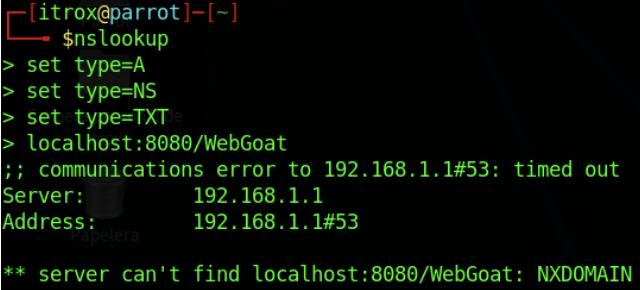
\includegraphics[width=12cm]{img/nslookup.png}
                \vspace{0.1em}
                
                Fig. 1: Output por consola de nslookup
            \end{center}
            
            \newpage
    
            \hspace{20pt}
            Debido a que el servicio corresponde a un entorno local y no posee un dominio real establecido, la herramienta nos entrega un output por consola indicando que el nombre del dominio ingresado no existe en el directorio DNS (NXDOMAIN).
            
            \vspace{2em}
            
            \item \textbf{Wappalyzer}
            
            \vspace{1em}
            
            \hspace{20pt}
            Con la extensión de navegador Wappalyzer se descubren las diferentes tecnologías utilizadas para levantar el entorno de WebGoat, entre las cuales se observan dos frameworks de Javascript (Backbone.js y Require.js), tres librerías de Javascript (JQuery v3.4.1, JQuery UI v 1.10.3 y Underscore.js) y un font script (Font awesome). Como lenguaje de programación se indentifica el uso de \textit{Javascript}.
            
            \vspace{2em}
            
            \begin{center}
                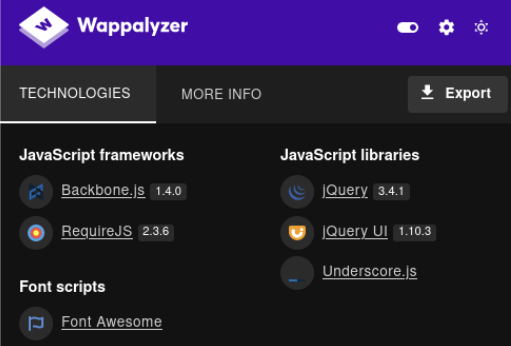
\includegraphics[width=12cm]{img/wappalyzer.png}
                \vspace{0.1em}
            
                Fig. 2: Información de Wappalyzer
            \end{center}
            
            \vspace{2em}
    
            \item \textbf{nmap}
            
            \vspace{1em}
            
            \newline
            \hspace{20pt}
            Se realiza escaneo mediante herramienta \textit{nmap}, con el fin de obtener información del sistema objetivo, tomando en cuenta la exposición de puertos abiertos, servicios en ejecución y versiones de estos, entre otros. 
            
            \vspace{2em}
            
            \begin{center}
                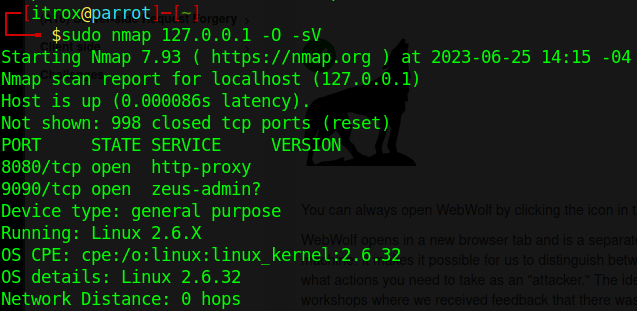
\includegraphics[width=12cm]{img/nmap.png}
                
                \vspace{0.1em}
                
                Fig. 3: Resultado de escaneo nmap
            \end{center}
            
            \vspace{2em}
            
            \begin{table}[H]
                \centering
                \begin{tabular}{|c|c|c|c|c|}
                     \hline % una linea horizontal
                     \textbf{PORT} & \textbf{Protocol} & \textbf{STATE} & \textbf{SERVICE} & \textbf{VERSION} \\
                     \hline % una linea horizontal
                     8080 & TCP & OPEN & http-proxy & - \\
                     \hline % una linea horizontal
                     9090 & TCP & OPEN & zeus-admin? & - \\
                     \hline % una linea horizontal
                \end{tabular}
                \caption{Estadísticas de servicios encontrados en escaneo nmap}
                \label{tab:my_label}
            \end{table}
            
            \vspace{1em}
    
            \newline
            \hspace{20pt}
            El servicio presenta los puertos 8080 y 9090 abiertos. En el primero encontramos corriendo la aplicación \textit{WebGoat} (URL "http://localhost:8080/WebGoat/start.mvc"), y en el segundo la aplicación \textit{WebWolf} (URL "http://localhost:9090"). Se utilizan los parámetros -sV (para obtener datos sobre versiones de los servicios que se ejecutan en cada puerto) y -O  (para obtener información del sistema operativo desde el que se ejecuta la aplicación web). Debido a que el protocolo de ambos puertos abiertos es TCP, se podría ingresar el comando -sS en la solicitud de nmap, con el fin de realizar un escaneo TCP/SYN sobre el servicio.
            
        \end{enumerate}
    \end{enumerate}
    \newpage





%%%%%%%%%%%%%%%%%%%%%%%%%%%%%%%%%%%%%%%%%%%%%%%%%%%%%%%
%%%%%2. Explotación de vulnerabilidades detectadas%%%%%
%%%%%%%%%%%%%%%%%%%%%%%%%%%%%%%%%%%%%%%%%%%%%%%%%%%%%%%
\phantomsection
\newsection{2. Explotación de vulnerabilidades}

\vspace{2em}

\hspace{20pt}
En este capítulo se lleva a cabo la investigación y análisis sobre las vulnerabilidades planteadas en el entorno de práctica \textit{WebGoat}. Entre ellas se verán SQLi, XSS, XXE entre otras.

\vspace{1em}

\begin{enumerate}
    \begin{enumerate}
        
        %%%%%%%%%%%%%%
        %%%% SQLi %%%%
        %%%%%%%%%%%%%%
        \item{\textbf{A3 Injection - SQL Injection (intro)}}
       
        \vspace{1em}

        %%%%%%%%%%%%%%%%%%
        %%%% Módulo 2 %%%%
        %%%%%%%%%%%%%%%%%%
        \textbf{Módulo 2}
        
        \vspace{1em}

        \hspace{20pt}
        La descripción del ejercicio solicita recuperar por pantalla el departamento al que pertenece el empleado Bob Franco. Tomando en cuenta esto se puede obtener la información de dos maneras:

        \vspace{1em}

            \begin{itemize}
                \item Obteniendo el departamento específico del usuario Bob Franco;
                \item Listando toda la información del usuario Bob Franco, entre la cual se encuentra su departamento.
            \end{itemize}

        \vspace{1em}

        \hspace{20pt}
        Para obtener específicamente el departamento al que pertenece Bob, se inyecta en el input type text que nos entrega la página la siguiente sentencia SQL:

        \vspace{1em}

        \begin{verbatim}
SELECT department FROM employees WHERE first_name = 'Bob';
        \end{verbatim}
        
        \hspace{20pt}
        La sentencia ingresada indica lo siguiente: \textit{"Indicar el contenido de la columna \textit{department} de la tabla \textit{employees}, en donde el valor de la columna \textit{first name} sea Bob"}. Así, se obtiene el siguiente resultado:

        \newpage

        \begin{center}
            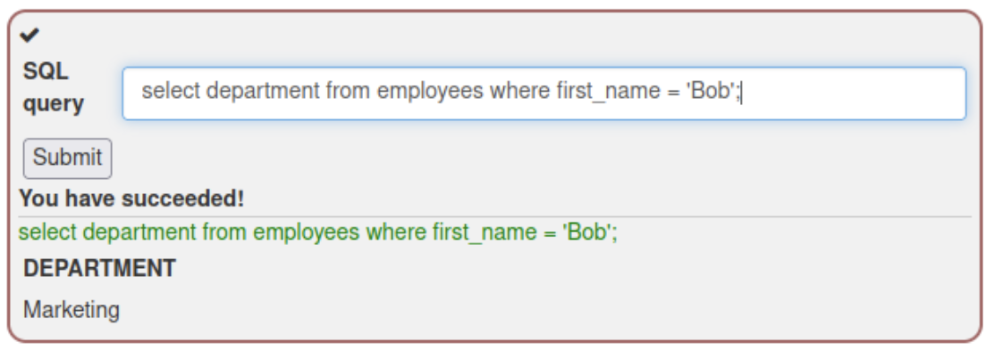
\includegraphics[width=12cm]{img/sqli1.png}
            
            \vspace{0.1em}
            
            Fig. 4: Resultado sentencia SQL específica
        \end{center}
        
        \vspace{2em}

        \hspace{20pt}
        Por otro lado, para obtener por pantalla toda la información del usuario Bob, se inyecta:

        \vspace{1em}

        \begin{verbatim}
SELECT * FROM employees WHERE first_name = 'Bob';
        \end{verbatim}

        la cual es similar a la anterior, pero en este caso se solicita todo el contenido de la fila donde \textit{first name} sea Bob, con el caracter \textit{*}.

        \vspace{2em}
        
        \begin{center}
            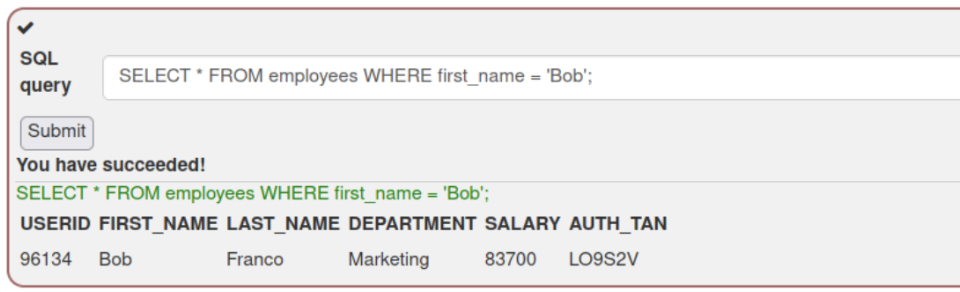
\includegraphics[width=12cm]{img/sqli2.png}
            
            \vspace{0.1em}
            
            Fig. 5: Resultado sentencia SQL general
        \end{center}

        \vspace{2em}
        
        \hspace{20pt}
        Del proceso anterior, se obtiene que el departamento del usuario Bob Franco es \textit{Marketing}.
        
        \newpage

        %%%%%%%%%%%%%%%%%%
        %%%% Módulo 3 %%%%
        %%%%%%%%%%%%%%%%%%
        \textbf{Módulo 3}
        
        \vspace{1em}

        \hspace{20pt}
        En esta ocasión se solicita cambiar de departamento al usuario Tobi Barnett hacia \textit{Sales}. Para realizar esta modificación se ingresa la sentencia SQL:

        \vspace{1em}

        \begin{verbatim}
UPDATE employees SET department='Sales' WHERE first_name = 'Tobi';
        \end{verbatim}

        \hspace{20pt}
        \textit{"Actualizar contenido en tabla employees para la columna \textit{department}. Asignar valor Sales cuando la columna first name sea Tobi"}. Tras hacer esto, se obtiene por pantalla lo siguiente:

        \vspace{2em}

        \begin{center}
            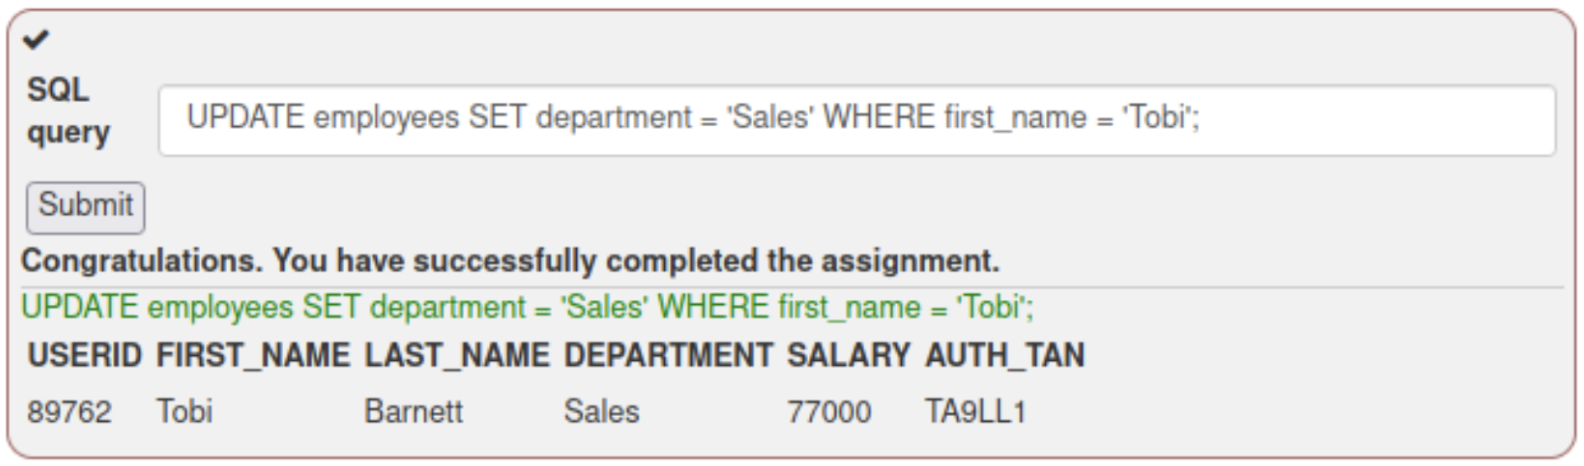
\includegraphics[width=12cm]{img/sqli3.png}
            
            \vspace{0.1em}
            
            Fig. 6: Resultado sentencia SQL cambio de departamento
        \end{center}
        
        \vspace{2em}

        %%%%%%%%%%%%%%%%%%
        %%%% Módulo 4 %%%%
        %%%%%%%%%%%%%%%%%%
        \textbf{Módulo 4}
        
        \vspace{1em}

        \hspace{20pt}
        Este módulo solicita la modificación del esquema base en la tabla \textit{employees}, añadiendo una nueva columna llamada \textit{phone}. Para realizar esta acción se utilizan los comandos SQL \textit{ALTER} y \textit{ADD}, los cuales permiten alterar el contenido de una tabla específica, añadiendo o elimando columnas (en este caso se añade una mediante \textit{ADD}). A esta nueva columna se le asigna la característica de poder albergar por casilla un máximo de 20 caracteres mediante el argumento \textit{varchar(20)}:

        \vspace{1em}

        \begin{verbatim}
ALTER TABLE employees ADD phone varchar(20);
        \end{verbatim}

        \newpage

        \begin{center}
            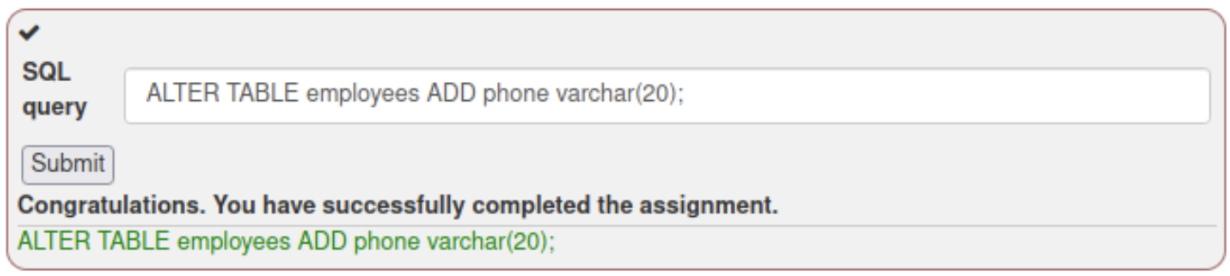
\includegraphics[width=12cm]{img/sqli4.png}
            
            \vspace{0.1em}
            
            Fig. 7: Resultado sentencia SQL ingreso de nueva columna a tabla
        \end{center}
        
        \vspace{2em}

        %%%%%%%%%%%%%%%%%%
        %%%% Módulo 5 %%%%
        %%%%%%%%%%%%%%%%%%
        \textbf{Módulo 5}
        
        \vspace{1em}

        \hspace{20pt}
        Ahora, se solicita conceder derechos de acceso a la tabla \textit{grant rights} al usuario \textit{unauthorized user}. Para esto se ingresa la sentencia:

        \vspace{1em}

        \begin{verbatim}
GRANT ALL ON grant_rights TO unauthorized_user;
        \end{verbatim}

        \hspace{20pt}
        Mediante \textit{GRANT ALL ON} se asigna el permiso de acceso a una tabla a un usuario específico designado por \textit{TO}. Por pantalla se obtiene como resultado la correcta ejecución de la sentencia SQL:
        
        \vspace{2em}

        \begin{center}
            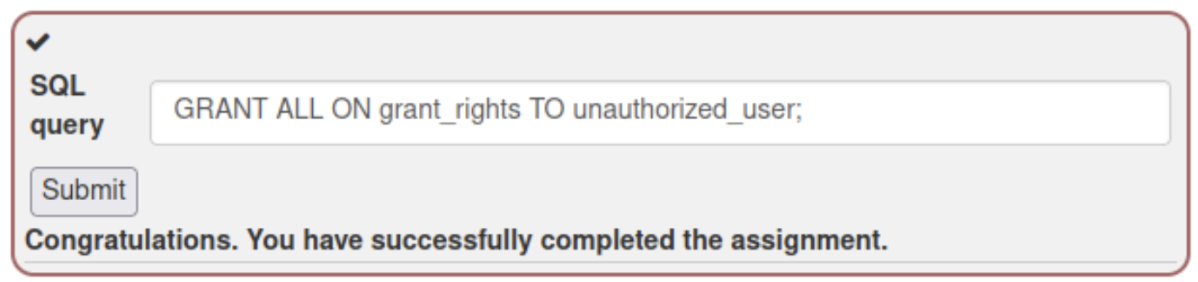
\includegraphics[width=12cm]{img/sqli5.png}
            
            \vspace{0.1em}
            
            Fig. 8: Resultado sentencia SQL asignación de permisos
        \end{center}
        
        \vspace{2em}

        %%%%%%%%%%%%%%%%%%
        %%%% Módulo 9 %%%%
        %%%%%%%%%%%%%%%%%%
        \textbf{Módulo 9}
        
        \vspace{1em}

        \hspace{20pt}
        Tomando en cuenta los módulos anteriores, se solicita obtener todos los datos de la tabla \textit{users}, teniendo en cuenta la siguiente sentencia SQL como inicio:

        \vspace{1em}
        
        \begin{verbatim}
SELECT * FROM user_data WHERE first_name = 'John' AND last_name 
= '" + lastName + "';
        \end{verbatim}

        \newpage
        
        \hspace{20pt}
        De las opciones planteadas en la aplicación WebGoat se escoje

        \vspace{1em}
        
        \begin{verbatim}
Smith' OR '1' = '1
        \end{verbatim}

        ya que transforma la sentencia del inicio en la siguiente:

        \vspace{1em}
        
        \begin{verbatim}
SELECT * FROM user_data WHERE first_name = 'John' AND last_name
= ‘Smith’ or ‘1’ = ‘1’;
        \end{verbatim}

        la cual permite completar la sintaxis original de SQL (al no tener comilla simple al principio y al final, esta comienza y cierra los argumentos \textit{Smith} y \textit{1}, y no se generan errores por tener dos comillas simples en medio o al final de la sentencia). Por otro lado, al forzar un estado \textit{TRUE} mediante el booleano \textit{OR}, siempre se ejecutará la visualización del contenido de la tabla seleccionada porque uno de los dos argumentos siempre será verdadero (Tomando en cuenta que el planteamiento del ejercicio indica que no conocemos ningún nombre de usuario, ingresar \textit{Smith} o \textit{Roberto} entregará de igual manera el resultado).
        
        \vspace{2em}

        \begin{center}
            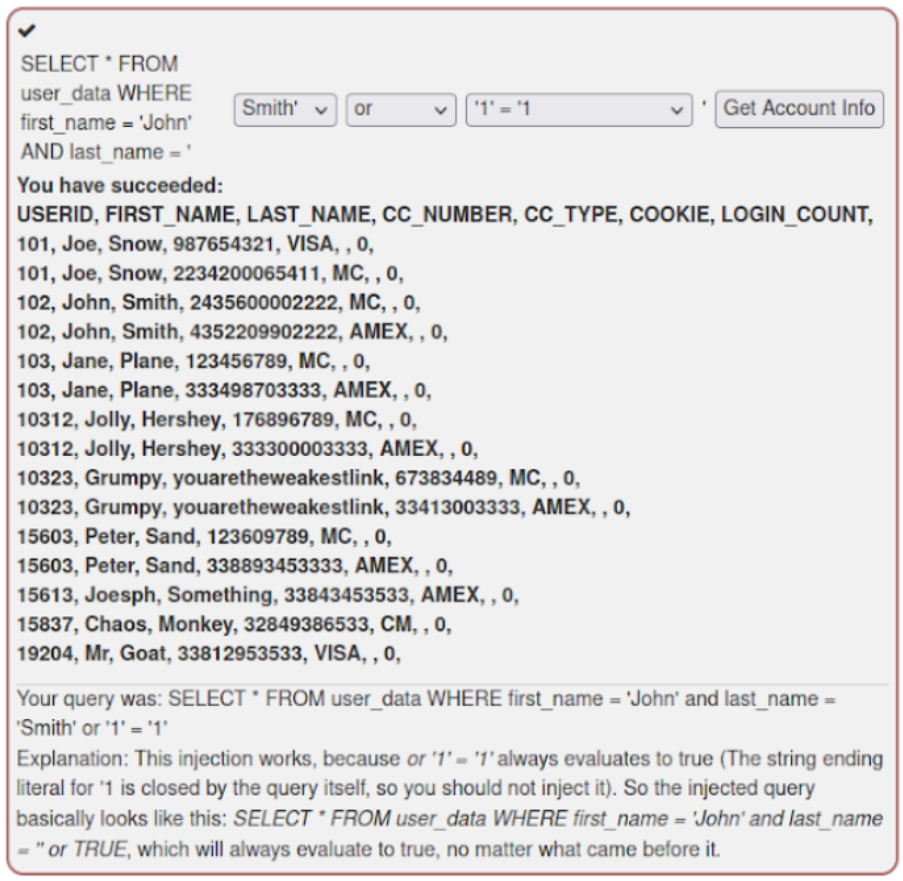
\includegraphics[width=10cm]{img/sqli6.png}
            
            \vspace{0.1em}
            
            Fig. 9: Resultado sentencia SQL visualización información de todos los usuarios
        \end{center}
        
        \newpage

        %%%%%%%%%%%%%%%%%%%
        %%%% Módulo 10 %%%%
        %%%%%%%%%%%%%%%%%%%
        \textbf{Módulo 10}
        
        \vspace{1em}

        \hspace{20pt}
        En este módulo se solicita obtener los mismos datos del módulo anterior, pero teniendo en cuenta que ahora los posibles campos susceptibles a inyecciones SQL son dos. Se comienza con la base de una sentencia SQL de la siguiente forma:

        \vspace{1em}
        
        \begin{verbatim}
SELECT * FROM user_data WHERE login_count = " + Login_Count +
" AND userid = " + User_ID;
        \end{verbatim}
        
        \hspace{20pt}
        Los campos con posibilidad de inyección son \textit{login count} y \textit{userid}. De las opciones planteadas por la aplicación se escoje la operación booleana

        \vspace{1em}
        
        \begin{verbatim}
0 or 1 = 1
        \end{verbatim}

        debido a que permite evaluar el argumento tanto de \textit{login count} como de \textit{userid}, el cual por la naturaleza de la operación booleana \textit{ OR 1 = 1}, generará siempre un resultado \textit{verdadero}. Esto permite poder mostrar el contenido de la tabla sea cual sea el valor con el que se compara la operación booleana nombrada anteriormente.

        \vspace{1em}
        
        \hspace{20pt}
        Se ingresa la operación como argumento de \textit{login count}, dejando una sentencia SQL de la siguiente forma:

        \vspace{1em}
        
        \begin{verbatim}
SELECT * FROM user_data WHERE login_count = 0 OR 1 = 1 AND userid= 0;
        \end{verbatim}

        Con esta sentencia no se aprecian resultados, lo cual indicaría en primera instancia que el campo de input text type \textit{login count} no es vulnerable a SQLi. Luego, se reemplaza la operación booleana como argumento de \textit{userid}. La sentencia resultante es:

        \vspace{1em}
        
        \begin{verbatim}
SELECT * FROM user_data WHERE login_count = 0 AND userid= 0 OR 1 = 1;
        \end{verbatim}

        Se confirma la vulnerabilidad SQLi mediante el campo \textit{userid}. Por pantalla obtenemos el resultado de toda la tabla \textit{usuarios}.

        \newpage
        
        \begin{center}
            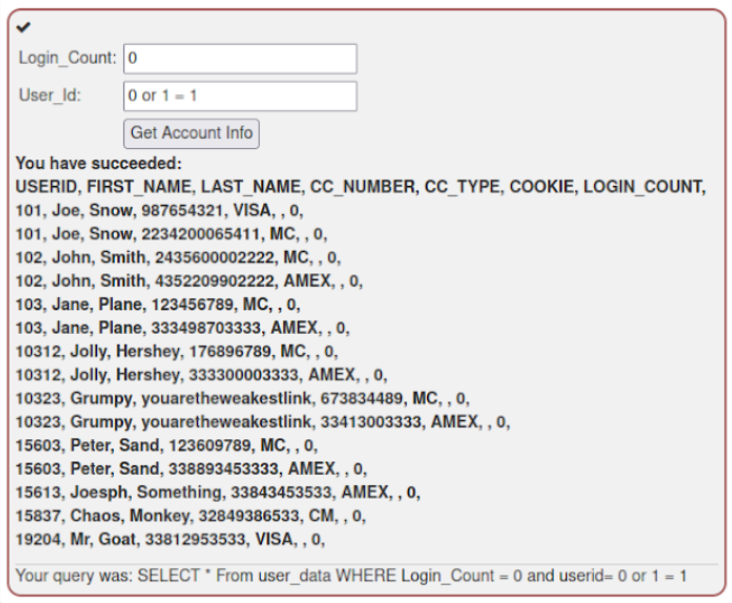
\includegraphics[width=12cm]{img/sqli7.png}
            
            \vspace{0.1em}
            
            Fig. 10: Resultado sentencia SQL visualización información de todos los usuarios segunda forma
        \end{center}
        
        \vspace{2em}

        %%%%%%%%%%%%%%%%%%%
        %%%% Módulo 11 %%%%
        %%%%%%%%%%%%%%%%%%%
        \textbf{Módulo 11}
        
        \vspace{1em}

        \hspace{20pt}
        Siendo el usuario \textit{John Smith}, se solicita obtener los datos de todos los usuarios pertenecientes a la tabla \textit{users} para conocer los salarios de estos. Cada usuario valida la revisión de sus datos mediante un número único de autenticación \textit{TAN}. Como consulta inicial se obtiene:

        \vspace{1em}
        
        \begin{verbatim}
"SELECT * FROM employees WHERE last_name = '" + name + "' AND auth_tan
= '" + auth_tan + "'";
        \end{verbatim}
        
        \hspace{20pt}
        Tras realizar la prueba de autenticación con nuestro usuario, se obtiene el siguiente resultado:

        \newpage
        
        \begin{center}
            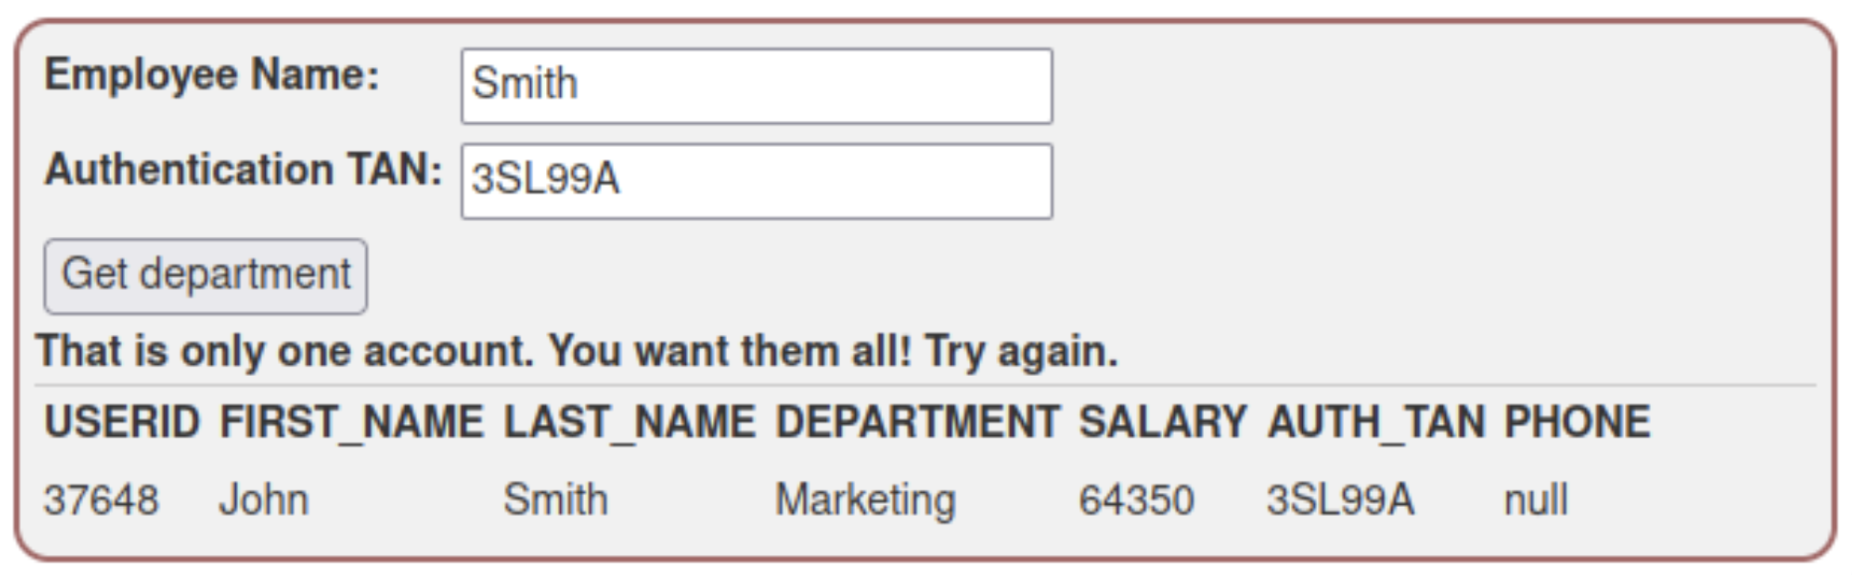
\includegraphics[width=12cm]{img/sqli8.png}
            
            \vspace{0.1em}
            
            Fig. 11: Resultado sentencia SQL validación código TAN
        \end{center}
        
        \vspace{2em}

        \hspace{20pt}
        Se inyecta la operación booleana \textit{' OR '1' = '1} en el campo \textit{Authentication TAN}, para confirmar la inyección SQL. Debido a que el campo vulnerable es \textit{Authentication TAN}, el ingresar o no algún tipo de valor en el campo \textit{Employee Name} es totalmente discriminante del resultado, tal y como se aprecia en la imagen del resultado:

        \vspace{2em}
        
        \begin{center}
            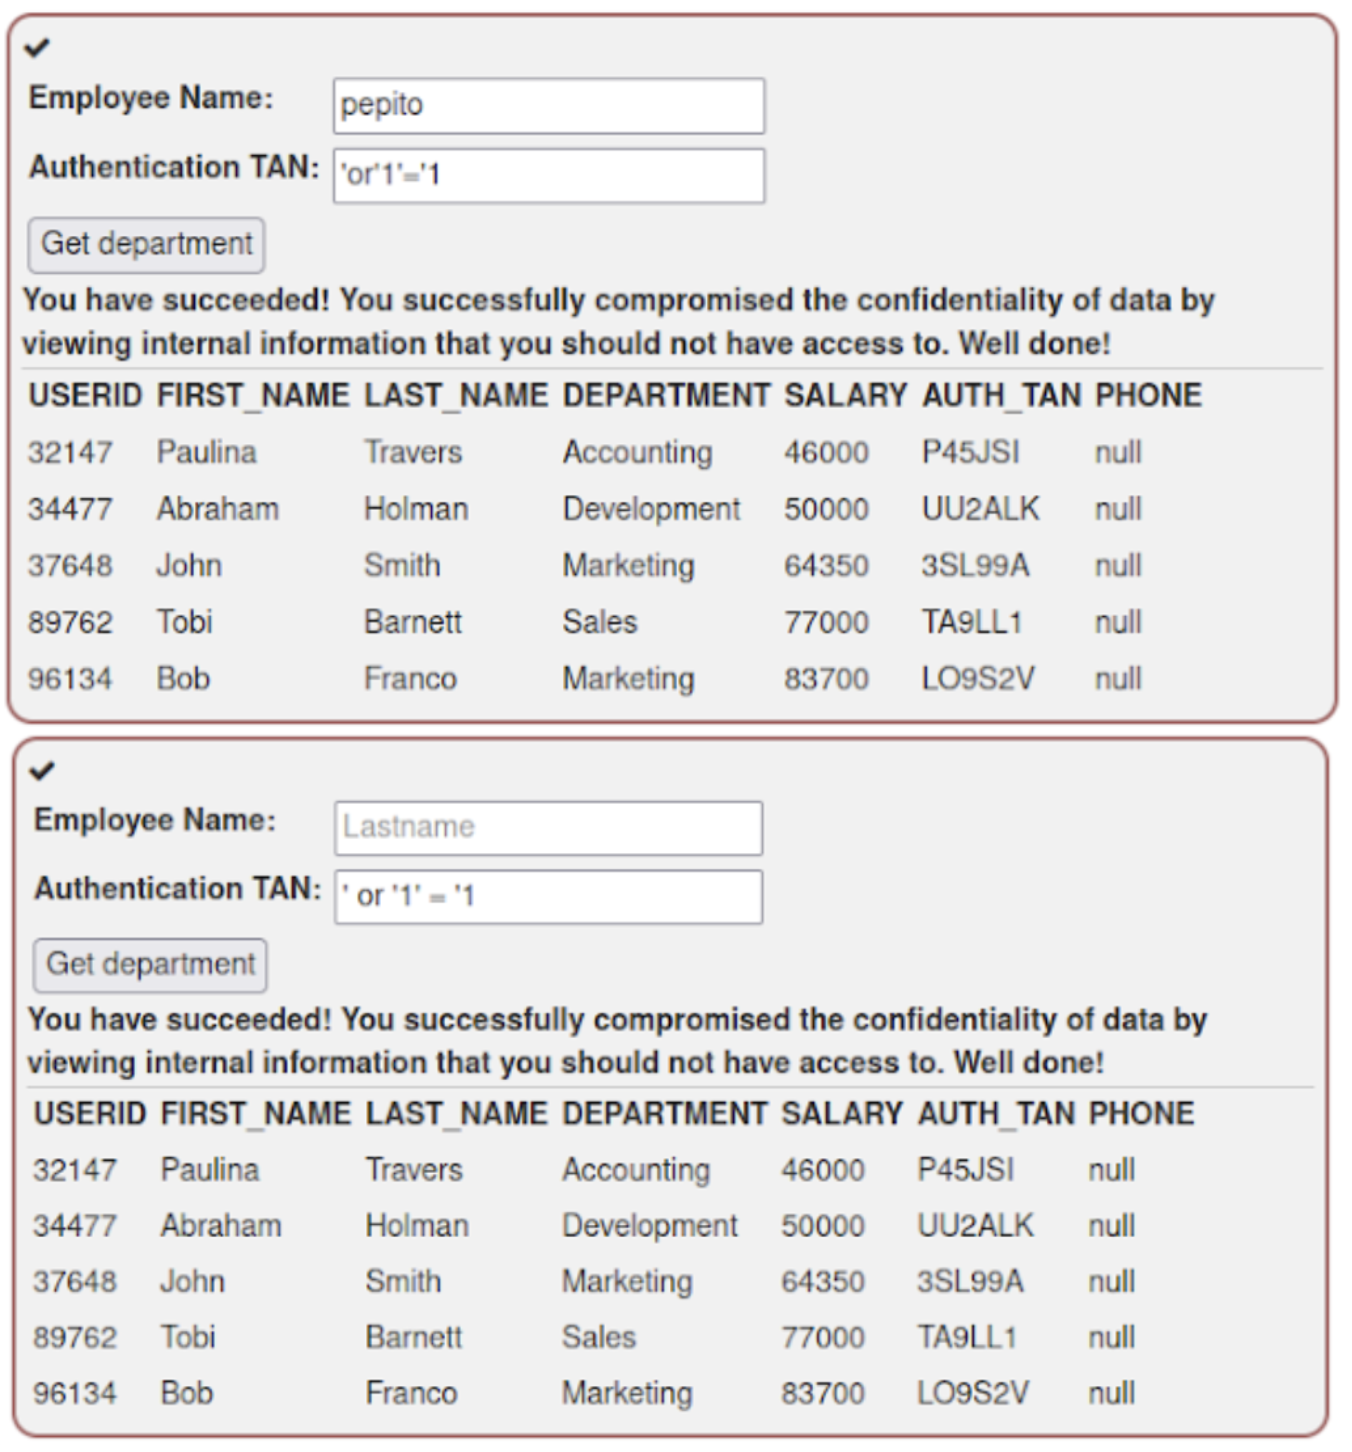
\includegraphics[width=11cm]{img/sqli9.png}
            
            \vspace{0.1em}
            
            Fig. 12: Resultado sentencia SQL datos de todos los usuarios
        \end{center}

        \newpage

        \hspace{20pt}
        Así, la sentencia SQL queda de la siguiente manera:
        
        \begin{verbatim}
SELECT * FROM employees WHERE last_name = 'pepito' AND auth_tan =
'1'or '1'='1';
        \end{verbatim}

        \vspace{2em}

        %%%%%%%%%%%%%%%%%%%
        %%%% Módulo 12 %%%%
        %%%%%%%%%%%%%%%%%%%
        \textbf{Módulo 12}
        
        \vspace{1em}

        \hspace{20pt}
        Con el módulo anterior se descubre que existen otros usuarios que tienen un mejor salario que el nuestro. Se solicita realizar un cambio en la base de datos con el fin de aumentar nuestro sueldo, modificando la columna \textit{Salary} de la tabla \textit{users}. Se utilizan los comandos SQL \textit{UPDATE} para actualizar la tabla seleccionada y \textit{SET}, para forzar el cambio de la columna indicada, cuando \textit{last name} tenga de valor a \textit{Smith}. Como base se utiliza la sentencia SQL del módulo anterior.

        \vspace{1em}

        \hspace{20pt}
        Para realizar esta acción tomamos en conocimiento que el campo vulnerable a SQLi es \textit{Authentication TAN}, e inyectamos lo siguiente:

        \vspace{1em}
        
        \begin{verbatim}
3SL99A'; UPDATE employees SET salary=99999 WHERE last_name = 'Smith
        \end{verbatim}
        
        \hspace{20pt}
        Esto con el fin de cerrar el argumento de \textit{auth tan} con \textit{3SL99A}' y concatenar mediante el caracter \textit{;} un comando en secuencia a la primera sentencia ejecutada. Como resulado se obtiene:

        \vspace{2em}
        
        \begin{center}
            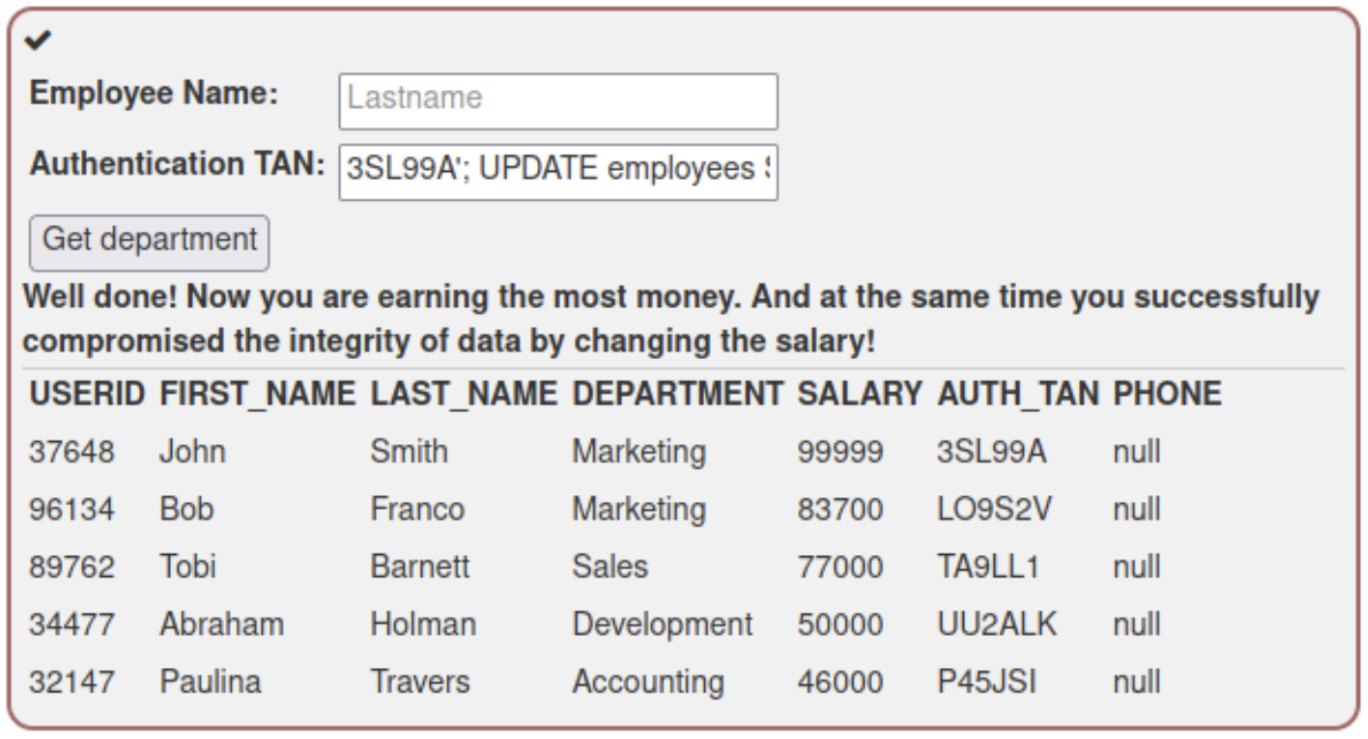
\includegraphics[width=12cm]{img/sqli10.png}
            
            \vspace{0.1em}
            
            Fig. 13: Resultado sentencia SQL concatenación de sentencia SQL
        \end{center}
        
        \newpage

        %%%%%%%%%%%%%%%%%%%
        %%%% Módulo 13 %%%%
        %%%%%%%%%%%%%%%%%%%
        \textbf{Módulo 13}
        
        \vspace{1em}

        \hspace{20pt}
        Finalmente, se debe eliminar la tabla \textit{access log} para borrar todo rastro de nuestro paso por la base de datos.

        \vspace{1em}

        \hspace{20pt}
        Se realiza la concatenación de un número \textit{1} en el campo de input en pantalla seguido de una comilla simple, con el fin de finalizar la sentencia. A esto se concatena el comando SQL \textit{DROP} para eliminar la tabla indicada. La sentencia final se ve de esta forma:

        \vspace{1em}
        
        \begin{verbatim}
1'; DROP TABLE access_log;
        \end{verbatim}
        
        \vspace{2em}
        
        \begin{center}
            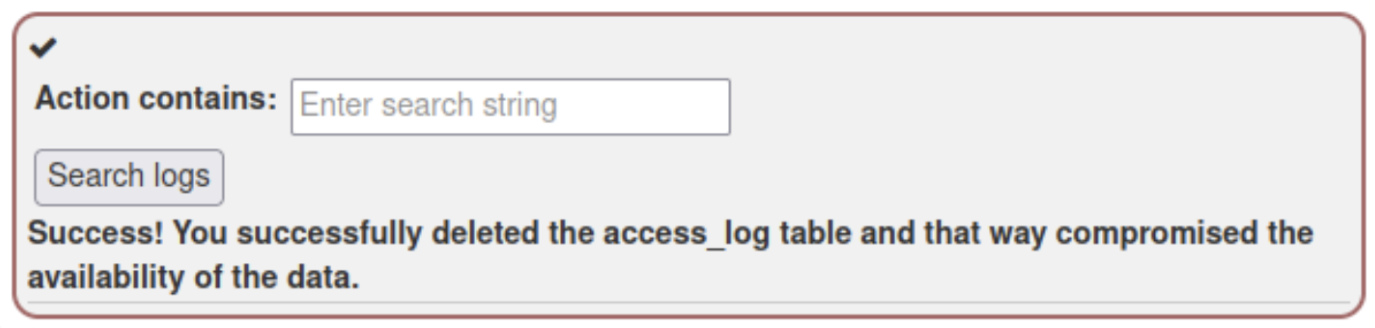
\includegraphics[width=12cm]{img/sqli11.png}
            
            \vspace{0.1em}
            
            Fig. 14: Resultado sentencia SQL eliminación de tabla de logs
        \end{center}
        
        \vspace{2em}

        %%%%%%%%%%%%%
        %%%% XSS %%%%
        %%%%%%%%%%%%%
        \item{\textbf{A3 Injection - Cross Site Scripting}}

        \vspace{1em}

        %%%%%%%%%%%%%%%%%%
        %%%% Módulo 2 %%%%
        %%%%%%%%%%%%%%%%%%
        \textbf{Módulo 2}
        
        \vspace{1em}

        \hspace{20pt}
        Se solicita revisar las cookies de la sesión desde dos herramientas distintas para corroborar similitud entre estas. Para realizar esto se utilizan 4 métodos, cada uno desde una ventana distinta del navegador:

        \vspace{1em}
        
            \begin{itemize}
                \item Utilizar las herramientas de desarrollador desde el apartado \textit{NETWORK}, y revisar una de las solicitudes presentes al recargar la sesión;
                \item Utilizar las herramientas de desarrollador desde el apartado \textit{CONSOLE} para ejecutar por pantalla una sentencia que entregue el ID de las cookies de sesión mediante \textit{alert};
                \item Utilizar las herramientas de desarrollador desde el apartado \textit{CONSOLE} para ejecutar por consola el valor de las cookies de sesión mediante el comando \textit{console.log};
                \item Secuestrando la solicitud \textit{GET} mediante un proxy (en este caso \textit{BURPSUITE}), y revisar la información de las cookies presente en dicha solicitud.
            \end{itemize}
        
        \vspace{1em}

        \hspace{20pt}
        Al obtener las cookies mediante las herramientas de desarrollador, apartado \textit{NETWORK}, se obtiene como ID de cookie de sesión:

        \vspace{1em}

        \begin{verbatim}
Cookie: JSESSION=xF1D_o7DZZvqlh3VOYRxOox-2gGA480RaTMK99jQ
        \end{verbatim}
        
        \vspace{2em} 
        
        \begin{center}
            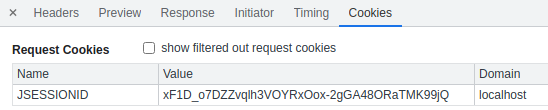
\includegraphics[width=12cm]{img/xss1.png}
            
            \vspace{0.1em}
            
            Fig. 15: Visualización cookies mediante herramientas de desarrollador, Network
        \end{center}
        
        \vspace{2em}

        \hspace{20pt}
        Luego, para obtener las cookies de sesión mediante las herramientas de desarrollador apartado \textit{CONSOLE} y emitir un pop-up message, se debe ingresar a consola el comando:
        
        \vspace{1em}

        \begin{verbatim}
alert(document.cookie);
        \end{verbatim}

        lo cual emite por pantalla:

        \vspace{2em}

        \begin{center}
            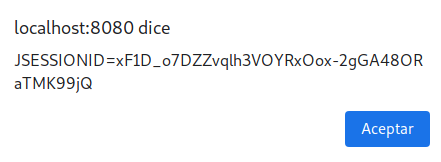
\includegraphics[width=12cm]{img/xss2.png}
            
            \vspace{0.1em}
            
            Fig. 16: Visualización cookies mediante herramientas de desarrollador, Console
        \end{center}
        
        \newpage

        \hspace{20pt}
        Ahora, para obtener las cookies de sesión mediante las herramientas de desarrollador apartado \textit{CONSOLE} por consola, se debe ingresar el comando:
        
        \vspace{1em}

        \begin{verbatim}
console.log(document.cookie);
        \end{verbatim}

        lo cual emite como output por consola:

        \vspace{2em}

        \begin{center}
            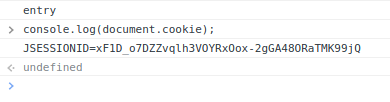
\includegraphics[width=12cm]{img/xss3.png}
            
            \vspace{0.1em}
            
            Fig. 17: Visualización cookies mediante herraemientas de desarrollador, Console
        \end{center}
        
        \vspace{2em}

        \hspace{20pt}
        Finalmente, obtener las cookies de sesión mediante un proxy implica interceptar una petición emitida al servidor antes de ser entregada. Esta acción se realiza con el software \textit{BURPSUITE}, haciendo uso de su herramienta \textit{Proxy}. Tras interceptar la petición, obtenemos la siguiente información:

        \vspace{2em}

        \begin{center}
            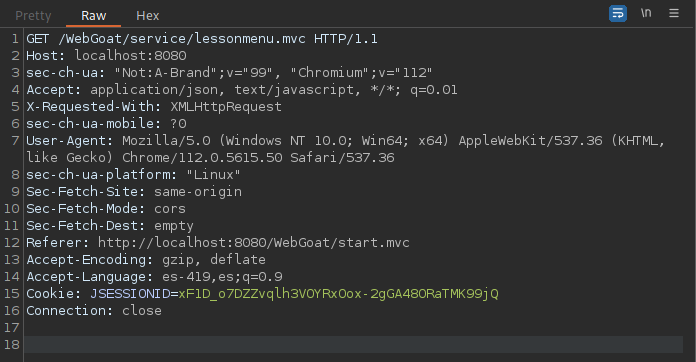
\includegraphics[width=12cm]{img/xss4.png}
            
            \vspace{0.1em}
            
            Fig. 18: Información obtenida por Burpsuite tras intercepción de solicitud GET
        \end{center}
        
        \newpage

        \hspace{20pt}
        Se puede observar que de todas las formas, y estando en diferentes ventanas del navegador, las cookies de sesión obtenidas son las mismas cuando se trata del mismo servicio.

        \vspace{2em}

        %%%%%%%%%%%%%%%%%%
        %%%% Módulo 7 %%%%
        %%%%%%%%%%%%%%%%%%
        \textbf{Módulo 7}
        
        \vspace{1em}

        \hspace{20pt}
        En este módulo se solicita identificar cual de los campos presentados por pantalla es susceptible a la vulnerabilidad \textit{XSS}. Esto se prueba inyectando código Javascript en cada uno de ellos mediante comandos \textit{alert}.

        \vspace{1em}

        \hspace{20pt}
        Tras realizar las pruebas se descubre que el input susceptible es \textit{Enter your code credit card number}. Se prueba ingresando el comando:

        \begin{verbatim}
<script>alert(“XSS”)</script>
        \end{verbatim}

        lo cual emite el pop-up message que se muestra a continuación:

        \vspace{2em} 
        
        \begin{center}
            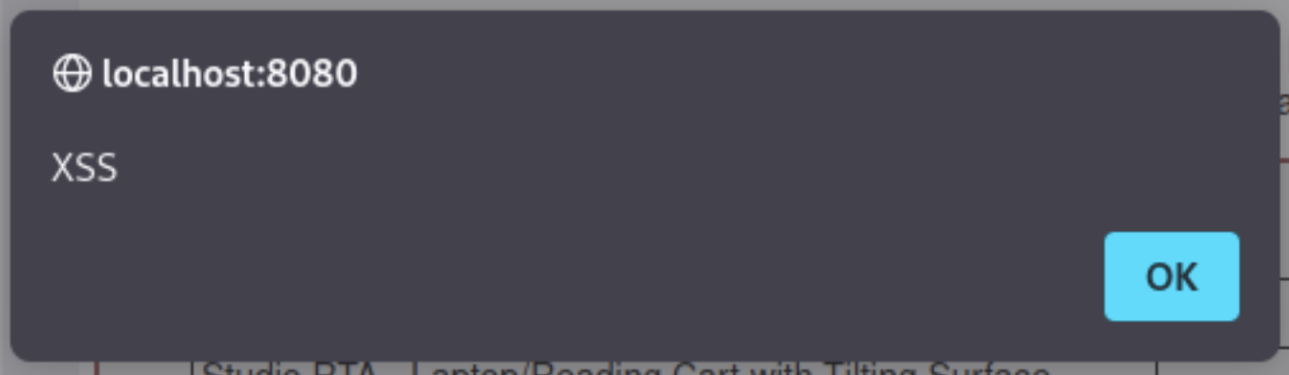
\includegraphics[width=12cm]{img/xss5.png}
            
            \vspace{0.1em}
            
            Fig. 19: Pop-up message visualizado por un XSS
        \end{center}
        
        \vspace{2em}

        \hspace{20pt}
        Tomando esto como referencia, se ejecuta el comando:
        
        \vspace{1em}

        \begin{verbatim}
<script>alert(document.cookie)</script>
        \end{verbatim}

        lo cual emite el pop-up message con las cookies de sesión:

        \newpage

        \begin{center}
            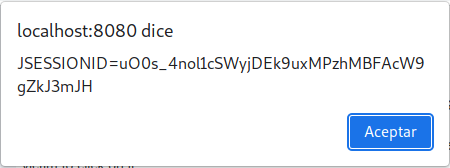
\includegraphics[width=12cm]{img/xss6.png}
            
            \vspace{0.1em}
            
            Fig. 20: Pop-up message visualizado por un XSS con valor de cookies de sesión
        \end{center}
        
        \vspace{2em}

        %%%%%%%%%%%%%%%%%%%
        %%%% Módulo 10 %%%%
        %%%%%%%%%%%%%%%%%%%
        \textbf{Módulo 10}
        
        \vspace{1em}

        \hspace{20pt}
        Se pide encontrar una ruta que tome entradas que se "reflejen" en la página, buscando en el directorio principal de esta. Mediante las herramientas de desarrollador apartado \textit{SOURCES}, se buscará una sentencia que llame al argumento de URL \textit{test} (la web-app usa backbone como su biblioteca primaria de JavaScript). Se toma en cuenta que a veces el código de prueba se deja en producción.
        
        \vspace{1em}

        \hspace{20pt}
        El objetivo principal es encontrar una ruta para \textit{test}, la cual pueda ser agregada a la ruta base

        \vspace{1em}

        \begin{verbatim}
/WebGoat/start.mvc#
        \end{verbatim}

        \hspace{20pt}
        Para realizar esto, se busca entre los documentos de la raíz de la página web, encontrando lo siguiente:

        \vspace{2em} 
        
        \begin{center}
            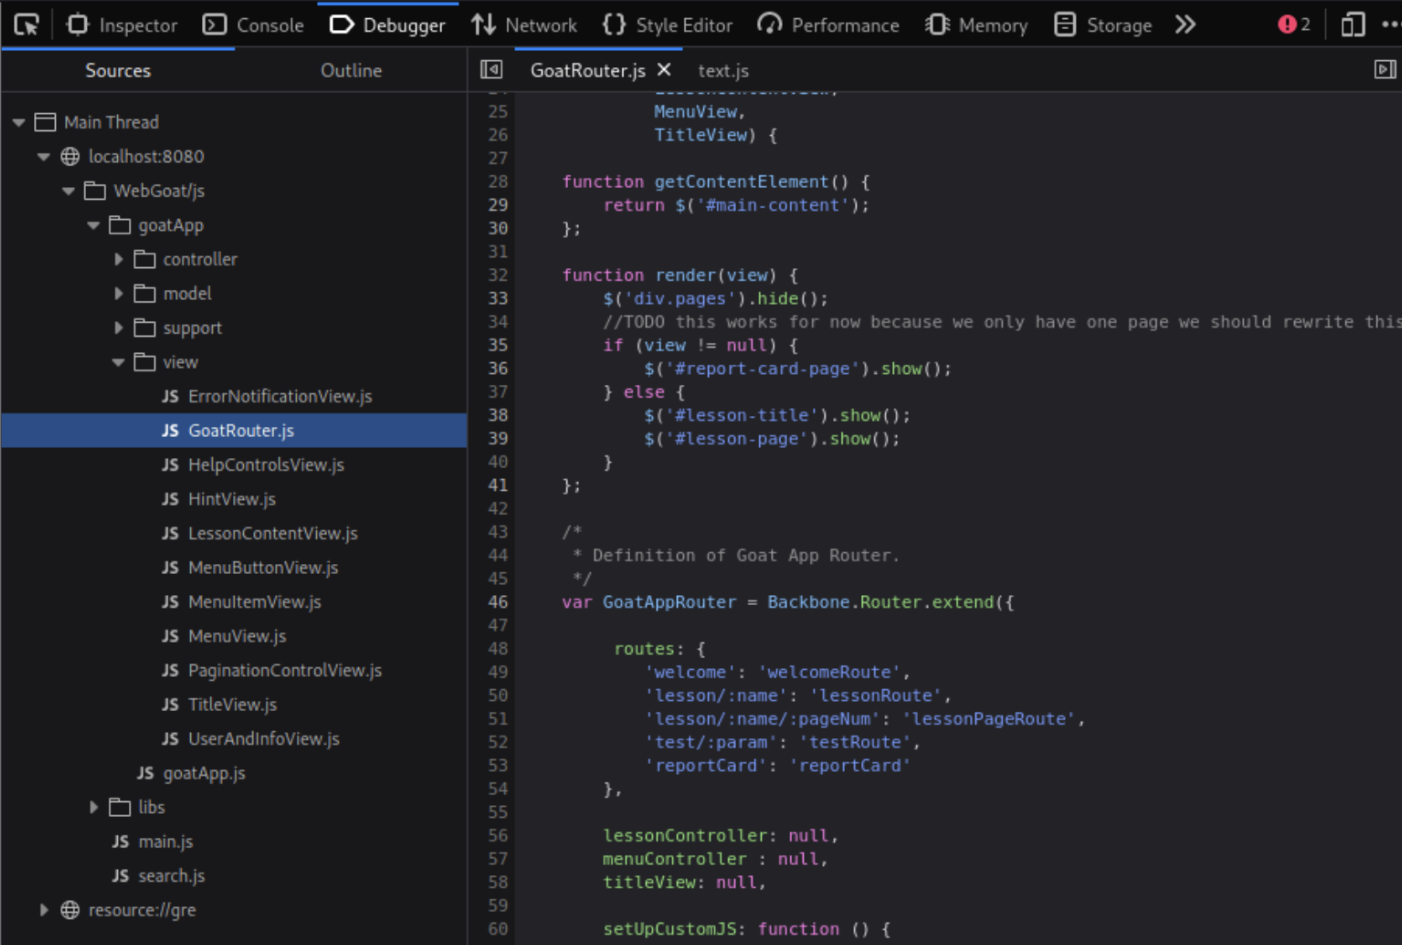
\includegraphics[width=12cm]{img/xss7.png}
            
            \vspace{0.1em}
            
            Fig. 21: Visualización herramientas de desarrollador, Sources
        \end{center}
        
        \vspace{2em}

        \begin{center}
            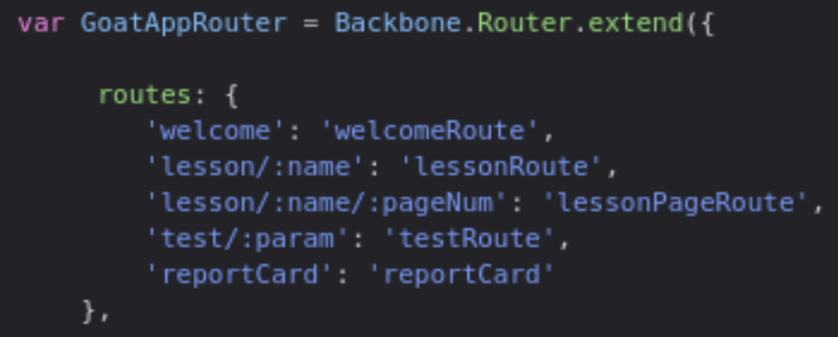
\includegraphics[width=12cm]{img/xss8.png}
            
            \vspace{0.1em}
            
            Fig. 22: Visualización herramientas de desarrollador, Sources, ruta a /test
        \end{center}
        
        \vspace{2em}

        \hspace{20pt}
        Con esto se obtiene \textit{/test} para incorporar a la ruta base, quedando esta de la siguiente manera:

        \vspace{1em}

        \begin{verbatim}
/WebGoat/start.mvc#/test
        \end{verbatim}

        \hspace{20pt}
        Finalmente, al ingresar la nueva ruta como argumento del input en pantalla, nos entrega el mensaje que el sitio a sido vulnerado.

        \newpage

        \begin{center}
            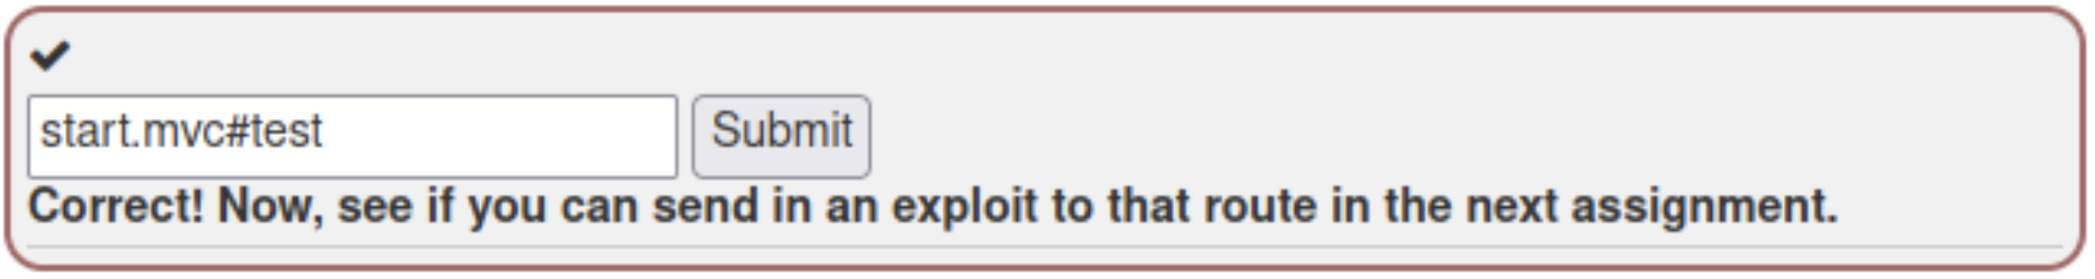
\includegraphics[width=12cm]{img/xss9.png}
            
            \vspace{0.1em}
            
            Fig. 23: Visualización ruta original con argumento /test
        \end{center}
        
        \vspace{2em}

        %%%%%%%%%%%%%%%%%%%
        %%%% Módulo 11 %%%%
        %%%%%%%%%%%%%%%%%%%
        \textbf{Módulo 11}
        
        \vspace{1em}

        \hspace{20pt}
        Se solicita usar la ruta encontrada en el módulo anterior y utilizarla para reflejar un parámetro de la ruta sin codificar, ejecutando una función interna en WebGoat. Esto con la finalidad de obtener un número aleatorio por consola que servirá como respuesta al módulo. Dicha función es:
        
        \vspace{1em}

        \begin{verbatim}
webgoat.customjs.phoneHome()
        \end{verbatim}

        \hspace{20pt}
        Se toma la URL original del servicio objetivo

        \begin{verbatim}
http://localhost:8080/WebGoat/start.mvc#
        \end{verbatim}

        y se agrega el argumento \textit{test} encontrado en el módulo 10. A esto se le incorpora como código Js la función nombrada anteriormente mediante script, generando la siguiente URL:

        \vspace{1em}

        \begin{verbatim}
http://localhost:8080/WebGoat/start.mvc#test/<script>webgoat.
customjs.phoneHome()</script>
        \end{verbatim}

        la cual al ejecutarse en el navegador queda de la siguiente forma:

        \vspace{1em}

        \begin{verbatim}
http://localhost:8080/WebGoat/start.mvc#test/%3Cscript%3Ewebgoat.
customjs.phoneHome()%3C%2fscript%3E
        \end{verbatim}
        
        y arroja el siguiente resultado:
        
        \newpage
        
        \begin{center}
            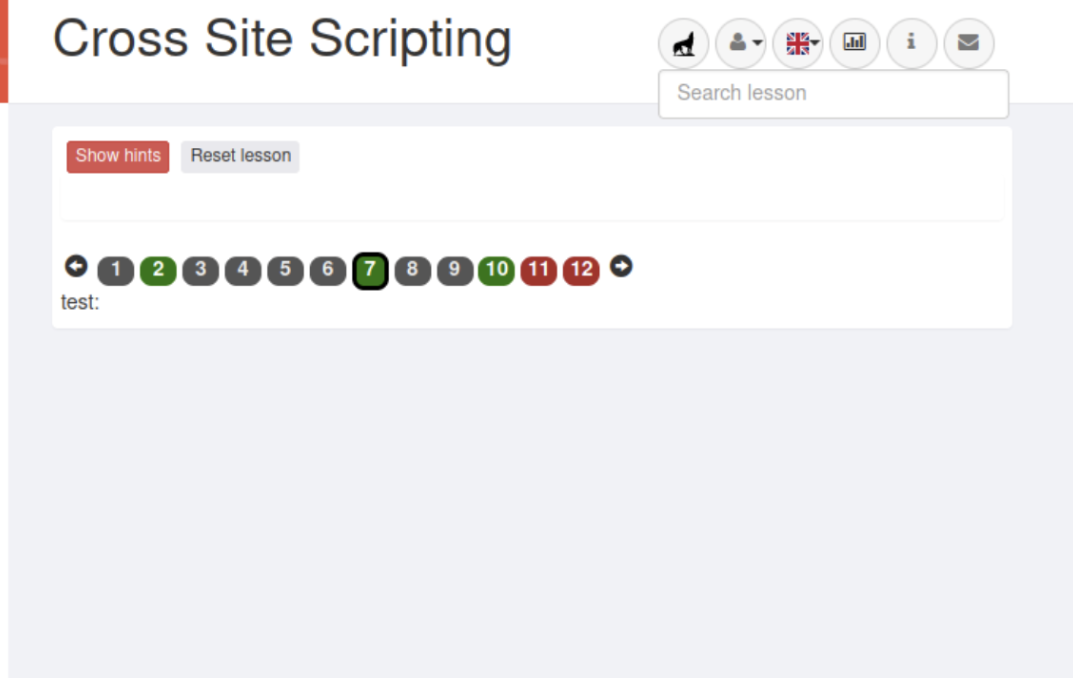
\includegraphics[width=12cm]{img/xss10.png}
            
            \vspace{0.1em}
            
            Fig. 24: Visualización ruptura por XXS
        \end{center}
        
        \vspace{2em}

        \hspace{20pt}
        Habiendo obtenido esto, se solicita la impresión por consola de las cookies de sesión, mediante el comando \textit{console.log(document.cookie);}. En el resultado emitido se observa el número buscado:

        \vspace{2em}

        \begin{center}
            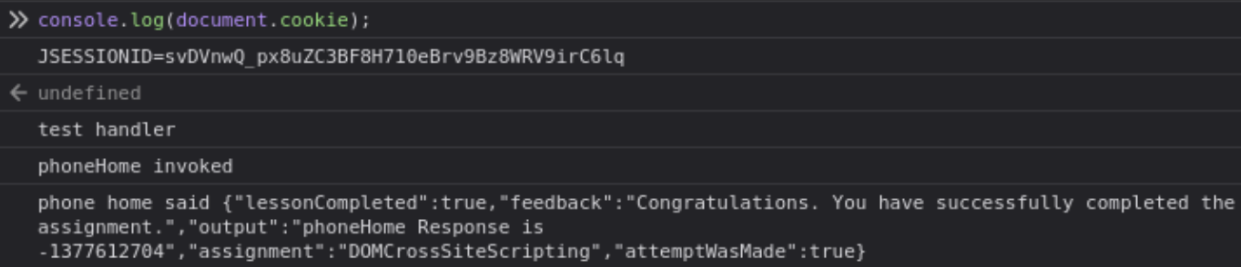
\includegraphics[width=12cm]{img/xss11.png}
            
            \vspace{0.1em}
            
            Fig. 25: Cookies obtenidas por herramientas de desarrollador, Console
        \end{center}
        
        \vspace{2em}

        \hspace{20pt}
        En este caso, el número de la respuesta es:
        
        \vspace{1em}

        \begin{verbatim}
-1377612704
        \end{verbatim}

        \begin{center}
            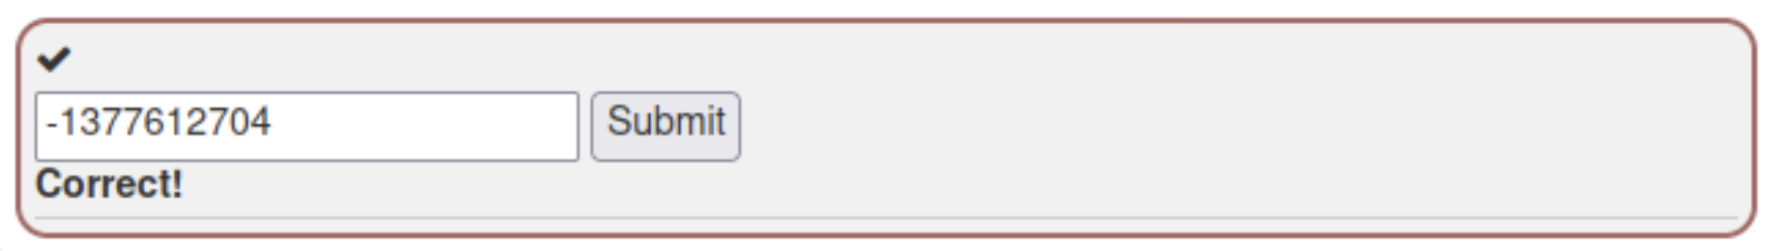
\includegraphics[width=12cm]{img/xss12.png}
            
            \vspace{0.1em}
            
            Fig. 26: Número de respuesta para vulnerabilidad XSS
        \end{center}
        
        \vspace{2em}

        %%%%%%%%%%%%%%%%%%%
        %%%% Módulo 12 %%%%
        %%%%%%%%%%%%%%%%%%%
        \textbf{Módulo 12}
        
        \vspace{1em}

        \hspace{20pt}
        Como módulo final de \textit{Cross Site Scripting} se plantea un quiz de 5 preguntas. Las respuestas se visualizan en las imagenes a continuación.
        
        \vspace{2em}

        \begin{center}
            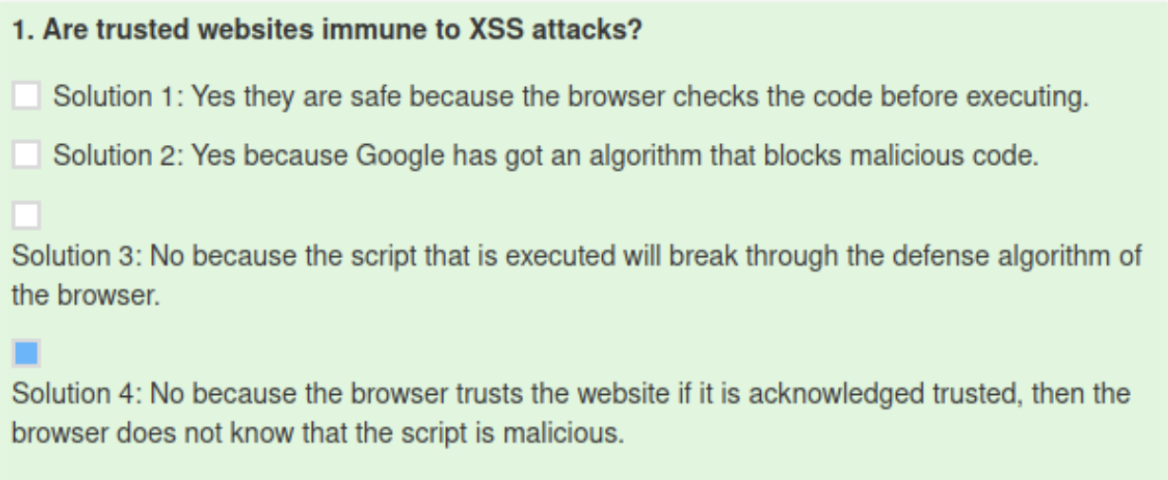
\includegraphics[width=12cm]{img/xss13.png}
            
            \vspace{0.1em}
            
            Fig. 27: Pregunta 1
        \end{center}
        
        \vspace{2em}

        \begin{center}
            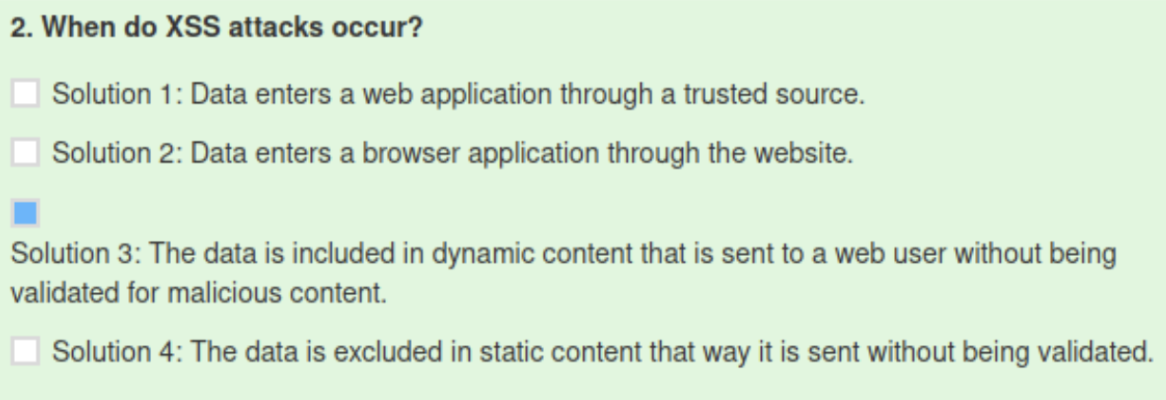
\includegraphics[width=12cm]{img/xss14.png}
            
            \vspace{0.1em}
            
            Fig. 28: Pregunta 2
        \end{center}
        
        \vspace{2em}

        \begin{center}
            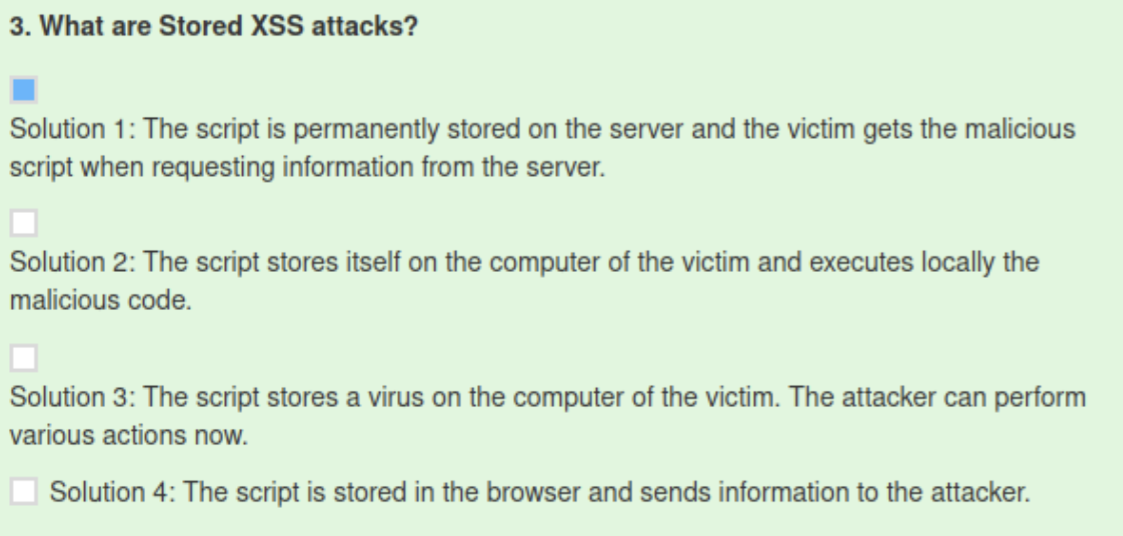
\includegraphics[width=12cm]{img/xss15.png}
            
            \vspace{0.1em}
            
            Fig. 29: Pregunta 3
        \end{center}
        
        \vspace{2em}

        \begin{center}
            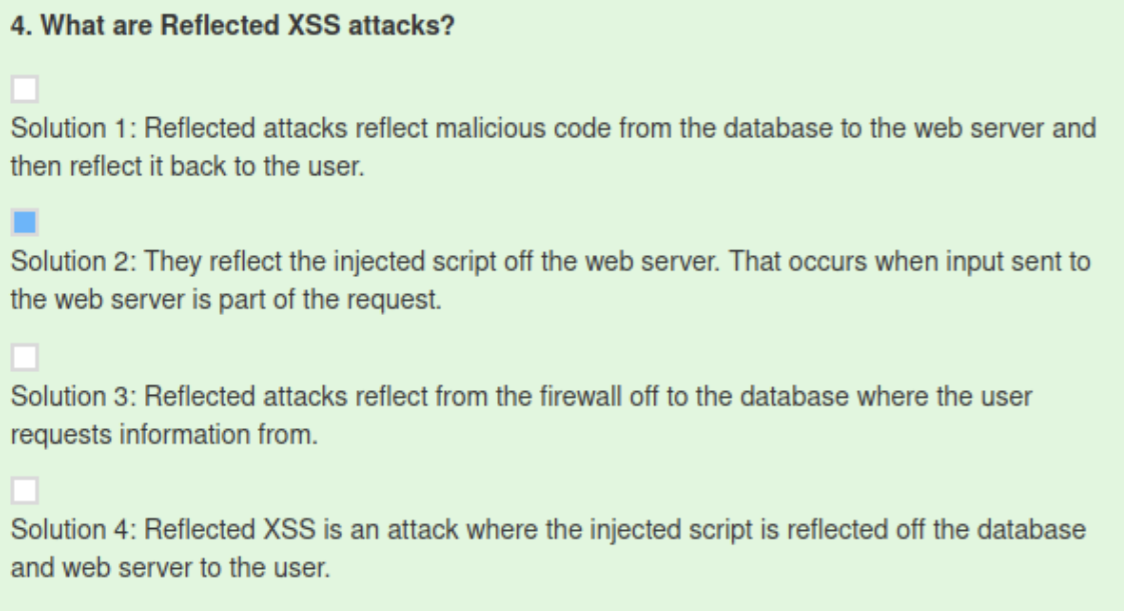
\includegraphics[width=12cm]{img/xss16.png}
            
            \vspace{0.1em}
            
            Fig. 30: Pregunta 4
        \end{center}
        
        \vspace{2em}

        \begin{center}
            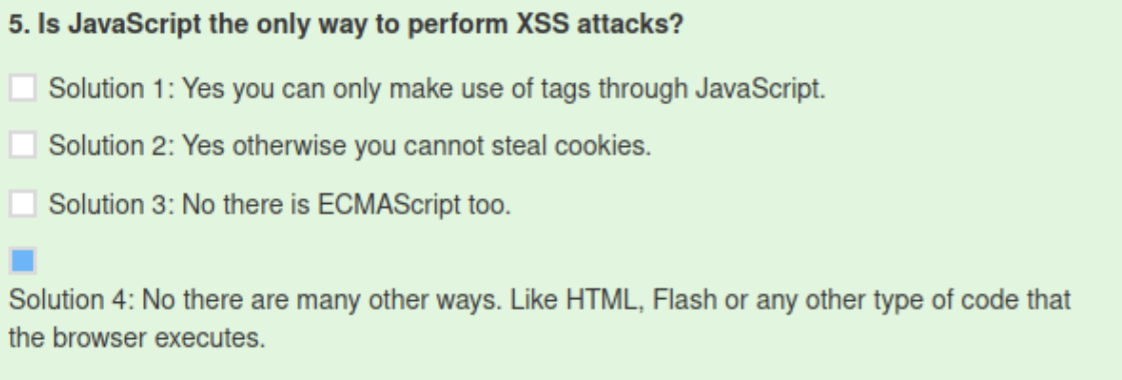
\includegraphics[width=12cm]{img/xss17.png}
            
            \vspace{0.1em}
            
            Fig. 31: Pregunta 5
        \end{center}
        
        \newpage






        %%%%%%%%%%%%%
        %%%% XXE %%%%
        %%%%%%%%%%%%%
        \item{\textbf{A5 Security Misconfiguration}}

        \vspace{1em}
        
        %%%%%%%%%%%%%%%%%%
        %%%% Módulo 4 %%%%
        %%%%%%%%%%%%%%%%%%
        \textbf{Módulo 4}
        
        \vspace{1em}

        \hspace{20pt}
        En este módulo se busca mediante el input del campo de comentarios, intentar una inyección XXE para listar por pantalla el contenido del directorio \textit{raíz} del sistema en donde se ejecuta la aplicación web.
        
        \vspace{1em}

        \hspace{20pt}
        Se comienza ingresando un comentario en el campo determinado
        
        \vspace{2em}

        \begin{center}
            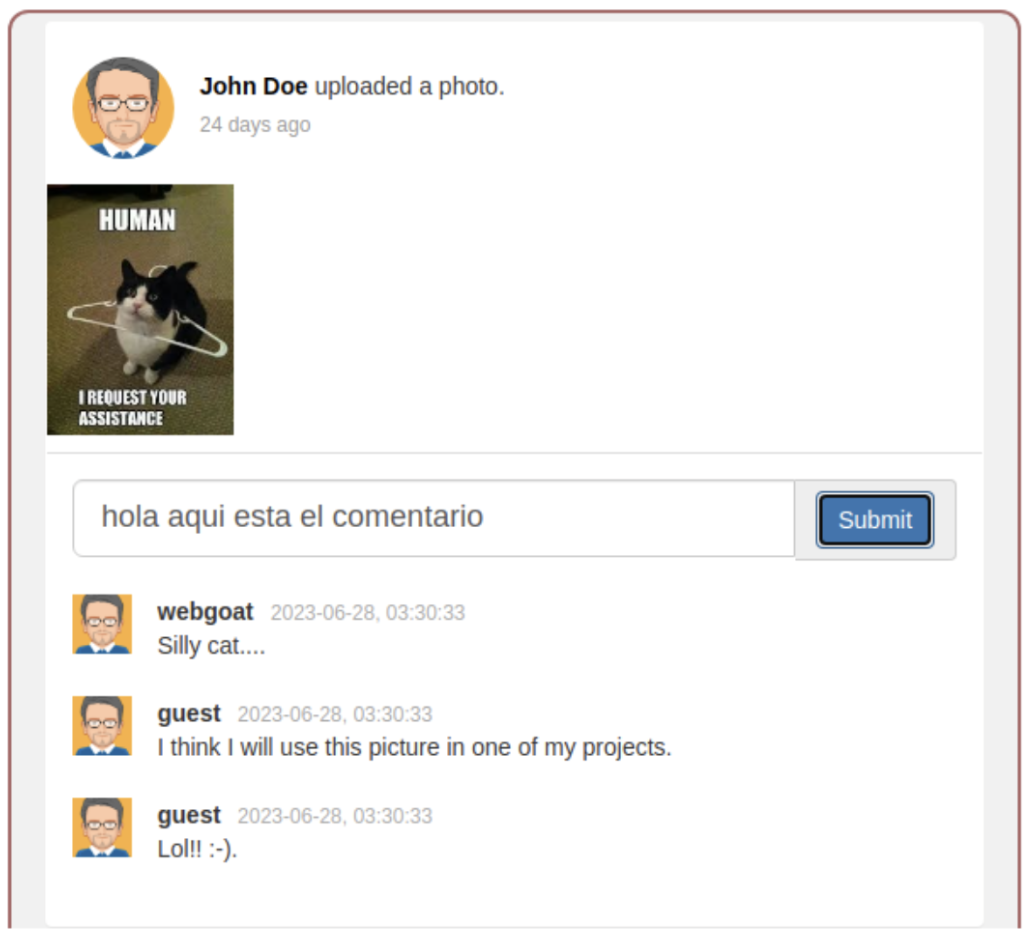
\includegraphics[width=12cm]{img/xxe0.png}
            
            \vspace{0.1em}
            
            Fig. 32: Sección comentarios XXE
        \end{center}
        
        \vspace{2em}

        \hspace{20pt}
        Luego, se realiza el secuestro de la solicitud mediante la herramienta proxy del software \textit{BURPSUITE}, del cual obtenemos la siguiente petición:

        \newpage

        \begin{center}
            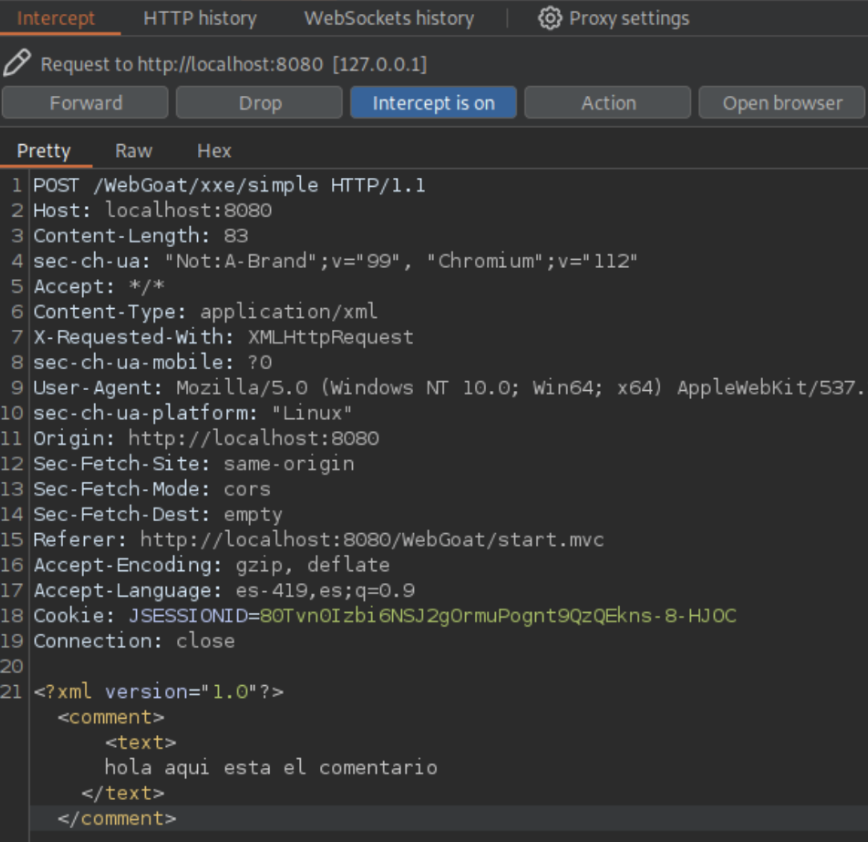
\includegraphics[width=12cm]{img/xxe1.png}
            
            \vspace{0.1em}
            
            Fig. 33: Petición POST interceptada por Burpsuite
        \end{center}
        
        \vspace{2em}

        \begin{verbatim}
<?xml version="1.0"?>
    <comment>
        <text>
            hola aquí esta el comentario
        </text>
    </comment>
        \end{verbatim}

        \hspace{20pt}
        Debido a que el campo de ingreso de comentarios en la página funciona bajo sentencias \textit{XML}, se realiza la modificación de su estructura para inyectar comandos de sistema y listar por pantalla un contenido específico de este. Se ingresa a la estructura \textit{XML} la declaración \textit{DOCTYPE}, la cual permite definir una estructura y proporcionar ciertas reglas de validación a la sentencia \textit{XML}. Así, se ingresa la declaración \textit{<!DOCTYPE replace [<!ENTITY xxe attack SYSTEM "file:///"> ]>} en la sentencia \textit{XML} original, generando:

        \newpage

        \begin{verbatim}
<?xml version="1.0"?>
    <!DOCTYPE replace [<!ENTITY xxe_attack SYSTEM "file:///"> ]>
    <comment>
        <text>
            &xxe_attack;
        </text>
    </comment>
        \end{verbatim}

        \vspace{2em}

        \begin{center}
            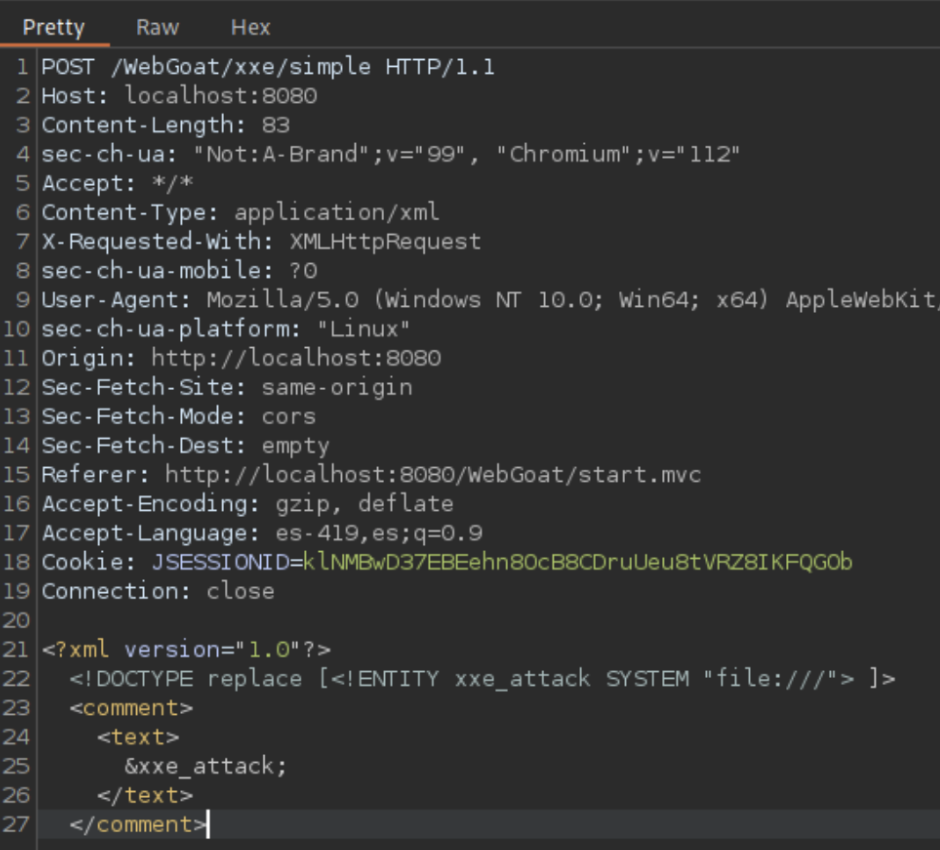
\includegraphics[width=12cm]{img/xxe2.png}
            
            \vspace{0.1em}
            
            Fig. 34: Nueva sintaxis XML en solicitud POST secuestrada por Burpsuite
        \end{center}
        
        \vspace{2em}

        \hspace{20pt}
        Se genera un DOCTYPE al cual se le asigna una entidad llamada \textit{xxe attack}. A dicha entidad se le atribuye el argumento \textit{file:///} con la finalidad de que al ser llamada a ejecución, se le asigne el contenido del argumento y sea este el que se ejecuta a nivel de sistema. Así, al llamar a ejecución a la entidad \textit{xxe attack}, lo que se ejecutará a nivel de sistema será \textit{file://}. Por otro lado, al argumento \textit{file://} se le asigna un tercer símbolo de \textit{/}, con el cual se hace referencia a la ubicación del directorio raíz del sistema.

        \newpage

        \hspace{20pt}
        Finalmente, en el apartado \textit{<comment>} se ingresa el nombre de la entidad creada en el DOCTYPE, pero entre los caracteres \textit{andpersand y ;}. Esto para dar a entender a la sentencia de que la entidad \textit{xxe attack} debe ejecutarse a nivel de sistema, y no ser ejecutado como un simple comentario por pantalla.

        \vspace{1em}

        \hspace{20pt}
        Tras esto, se libera la solicitud desde el proxy al servidor, obteniendo por pantalla el contenido del directorio raíz del sistema objetivo:

        \vspace{2em}

        \begin{center}
            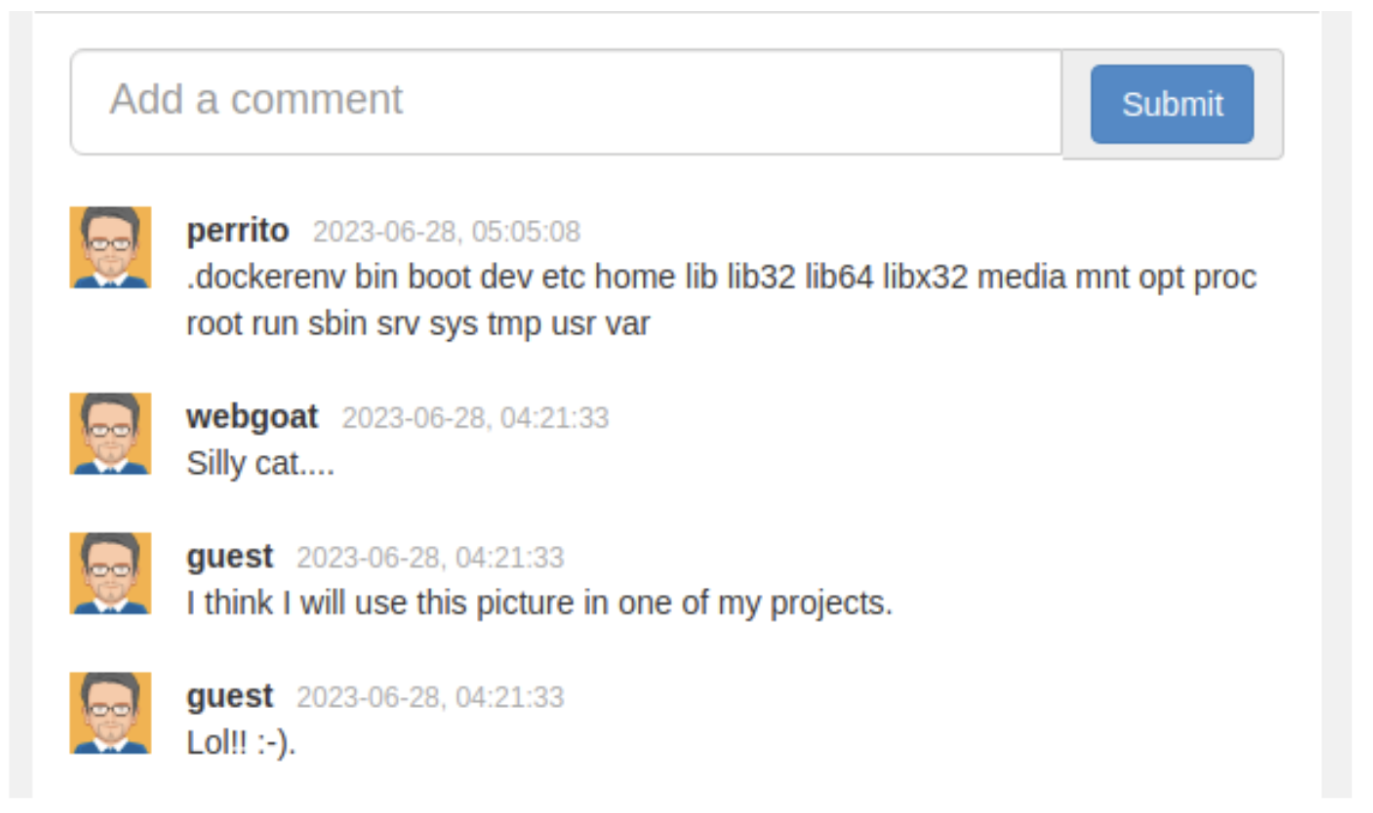
\includegraphics[width=12cm]{img/xxe3.png}
            
            \vspace{0.1em}
            
            Fig. 35: Visualización de directorios de ubicación raíz
        \end{center}

        \vspace{2em}

        \hspace{20pt}
        Comprobada la existencia de la vulnerabilidad, se procede a realizar pruebas para obtener información sensible del sistema, ingresando a ficheros como \textit{passwd}, \textit{shadow}, historial de consola, entre otros.

        \vspace{1em}
        
        \textbf{Fichero /etc/passwd}

        \vspace{1em}

        \begin{verbatim}
<?xml version="1.0"?>
    <!DOCTYPE replace [<!ENTITY xxe_attack SYSTEM "file:///etc/passwd"> ]>
        <comment>
            <text>
                &xxe_attack;
            </text>
        </comment>
        \end{verbatim}

        \newpage

        \begin{center}
            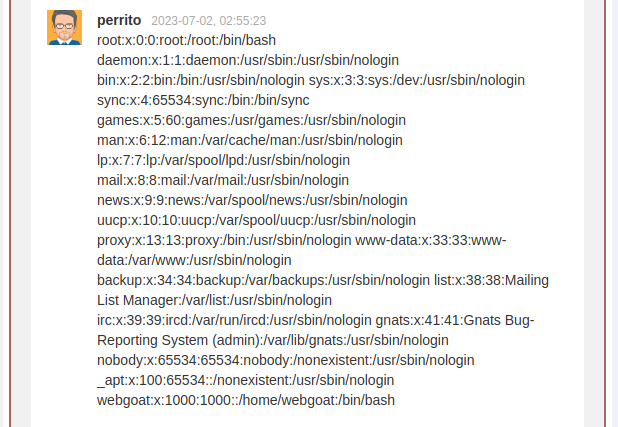
\includegraphics[width=12cm]{img/xxe10.png}
            
            \vspace{0.1em}
            
            Fig. 36: Fichero /etc/passwd
        \end{center}

        \vspace{2em}

        \textbf{Fichero /etc/shadow} (Debido a que el usuario que ejecuta el sistema es \textit{webgoat}, los ficheros shadow y sudoers no se pueden visualizar, ya que se necesitan permisos \textit{sudo} o ser usuario root para visualizarlo).

        \vspace{1em}

        \begin{verbatim}
<?xml version="1.0"?>
    <!DOCTYPE replace [<!ENTITY xxe_attack SYSTEM "file:///etc/shadow"> ]>
        <comment>
            <text>
                &xxe_attack;
            </text>
        </comment>
        \end{verbatim}

        \newpage

        \begin{center}
            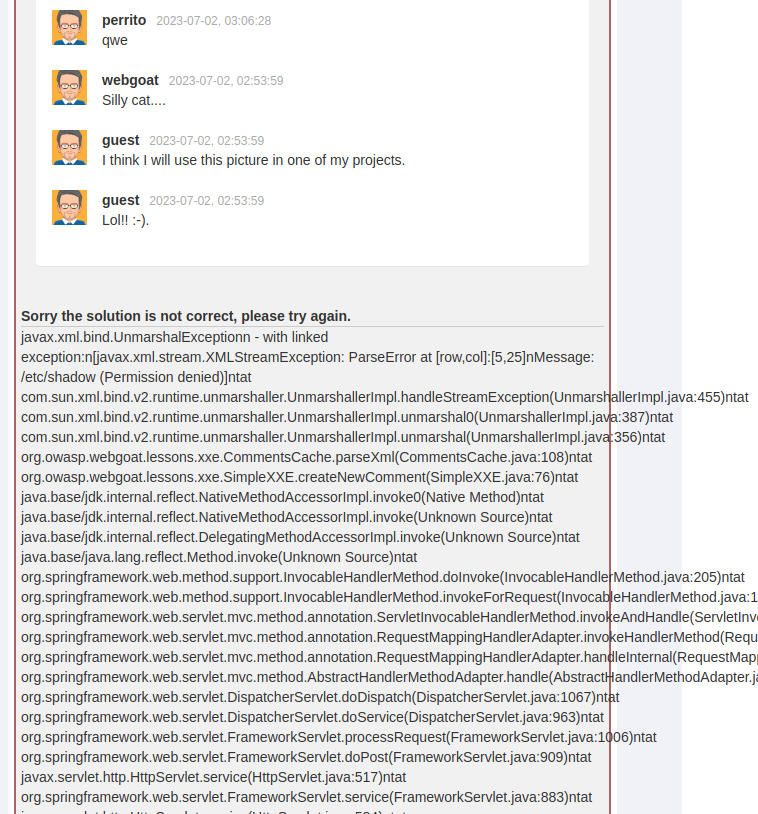
\includegraphics[width=12cm]{img/xxe11.png}
            
            \vspace{0.1em}
            
            Fig. 37: Fichero /etc/shadow
        \end{center}

        \vspace{2em}

        \textbf{Fichero /etc/hosts}

        \vspace{1em}

        \begin{verbatim}
<?xml version="1.0"?>
    <!DOCTYPE replace [<!ENTITY xxe_attack SYSTEM "file:///etc/hosts"> ]>
        <comment>
            <text>
                &xxe_attack;
            </text>
        </comment>
        \end{verbatim}

        \newpage

        \begin{center}
            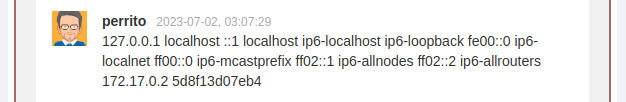
\includegraphics[width=12cm]{img/xxe12.png}
            
            \vspace{0.1em}
            
            Fig. 38: Fichero /etc/hosts
        \end{center}

        \vspace{2em}

        \textbf{Fichero /etc/shells}

        \vspace{1em}

        \begin{verbatim}
<?xml version="1.0"?>
    <!DOCTYPE replace [<!ENTITY xxe_attack SYSTEM "file:///etc/shells"> ]>
        <comment>
            <text>
                &xxe_attack;
            </text>
        </comment>
        \end{verbatim}

        \vspace{2em}

        \begin{center}
            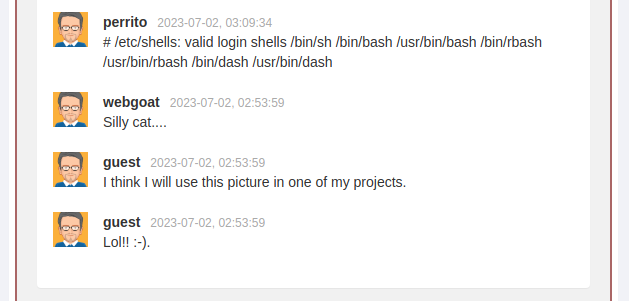
\includegraphics[width=12cm]{img/xxe13.png}
            
            \vspace{0.1em}
            
            Fig. 39: Fichero shells
        \end{center}

        \newpage

        \textbf{Directorio /var/log}

        \vspace{1em}

        \begin{verbatim}
<?xml version="1.0"?>
    <!DOCTYPE replace [<!ENTITY xxe_attack SYSTEM "file:///var/log/"> ]>
        <comment>
            <text>
                &xxe_attack;
            </text>
        </comment>
        \end{verbatim}

        \vspace{2em}

        \begin{center}
            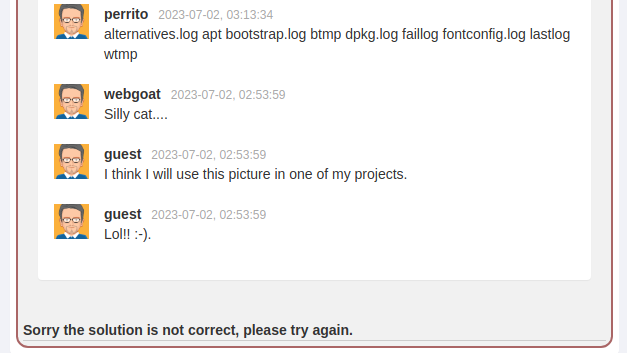
\includegraphics[width=12cm]{img/xxe14.png}
            
            \vspace{0.1em}
            
            Fig. 40: Directorio /var/log/
        \end{center}

        \vspace{2em}

        %%%%%%%%%%%%%%%%%%
        %%%% Módulo 7 %%%%
        %%%%%%%%%%%%%%%%%%
        \textbf{Módulo 7}
        
        \vspace{1em}

        \hspace{20pt}
        Se plantea realizar la misma inyección del módulo anterior, pero esta vez mediante un endpoint \textit{JSON}. Para esto, se secuestra la solicitud enviada al servidor de la misma forma que el módulo anterior:
        
        \newpage

        \begin{center}
            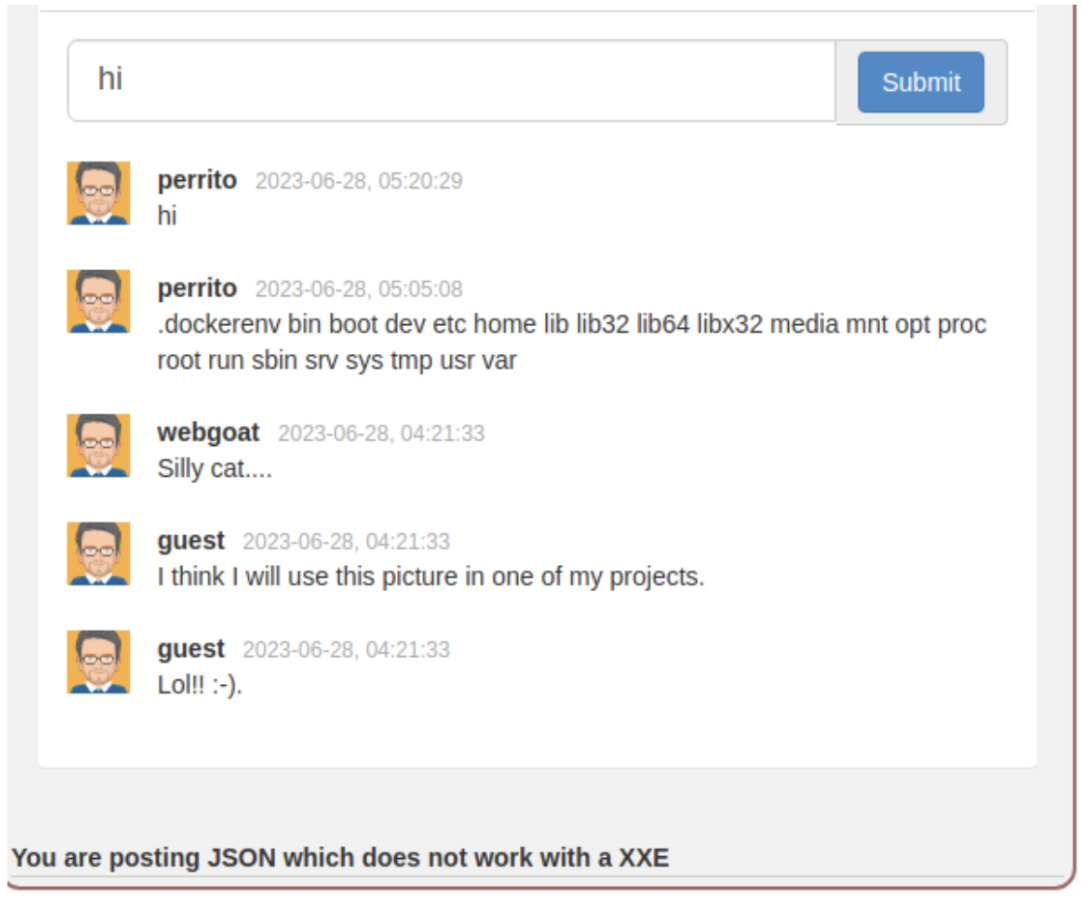
\includegraphics[width=12cm]{img/xxe4.png}
            
            \vspace{0.1em}
            
            Fig. 41: Pruebas inyección XXE en apartado comentarios
        \end{center}
        
        \vspace{2em}

        \begin{center}
            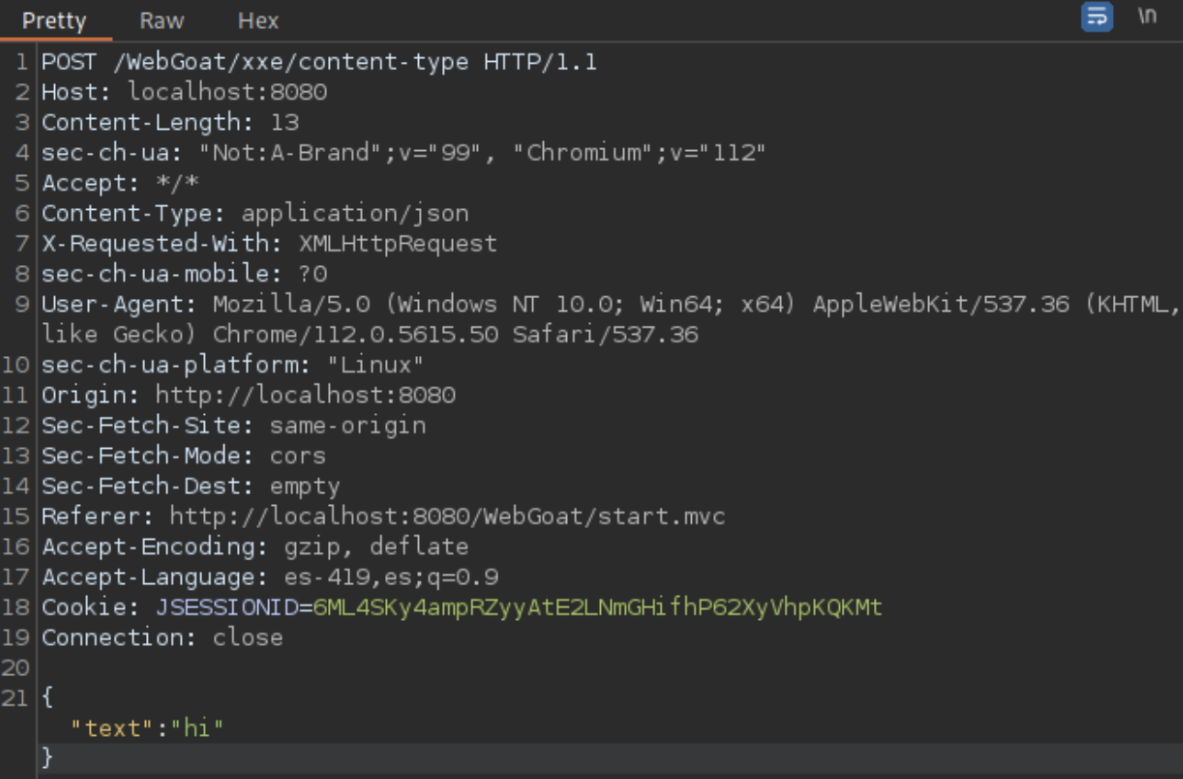
\includegraphics[width=12cm]{img/xxe5.png}
            
            \vspace{0.1em}
            
            Fig. 42: Petición intercetada por Burpsuite
        \end{center}
        
        \newpage

        \hspace{20pt}
        Se realiza el cambio del apartado \textit{Content-type} presente en la solicitud, pasando de tener \textit{application/json} a tener \textit{application/xml} como tipo de contenido. Luego en la sentencia \textit{json} se cambia su contenido por la sentencia \textit{xml} del módulo anterior. Esta vez se define una entidad llamada \textit{xxe}.

        \vspace{2em}

        \begin{center}
            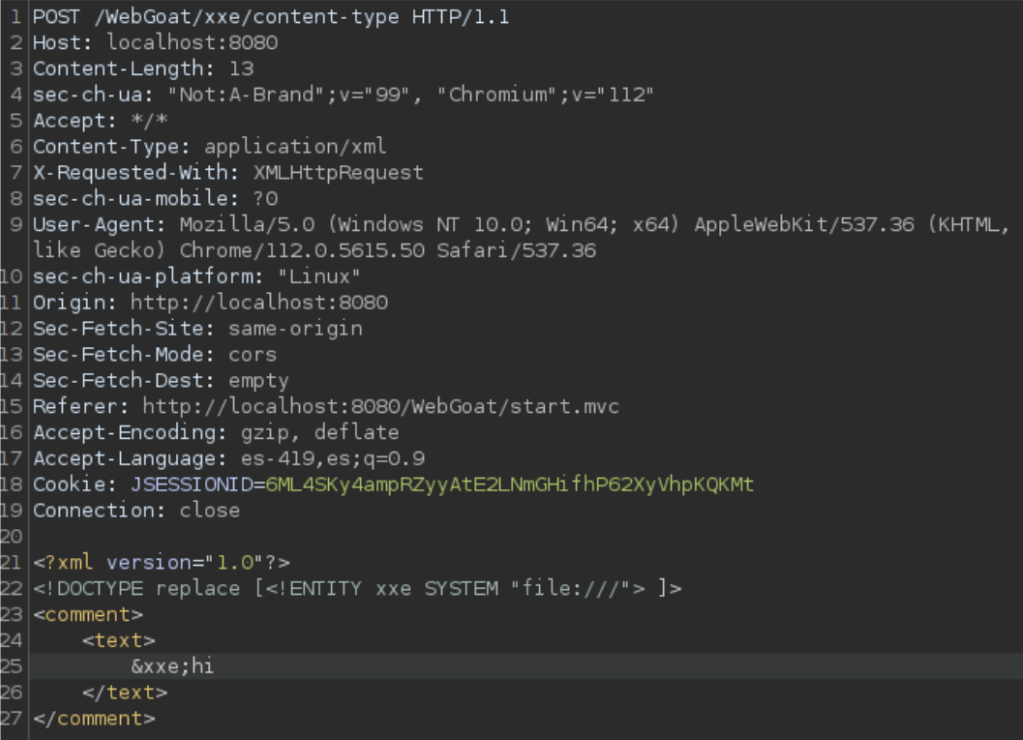
\includegraphics[width=12cm]{img/xxe6.png}
            
            \vspace{0.1em}
            
            Fig. 43: Petición interceptada y modificada a xml por Burpsuite
        \end{center}
        
        \vspace{2em}

        \hspace{20pt}
        Ya realizada la modificación en el cuerpo de la solictud secuestrada, se libera esta hacia el sevidor, lo cual permite obtener por pantalla nuevamente el contenido del directorio raíz del sistema objetivo.:

        \newpage

        \begin{center}
            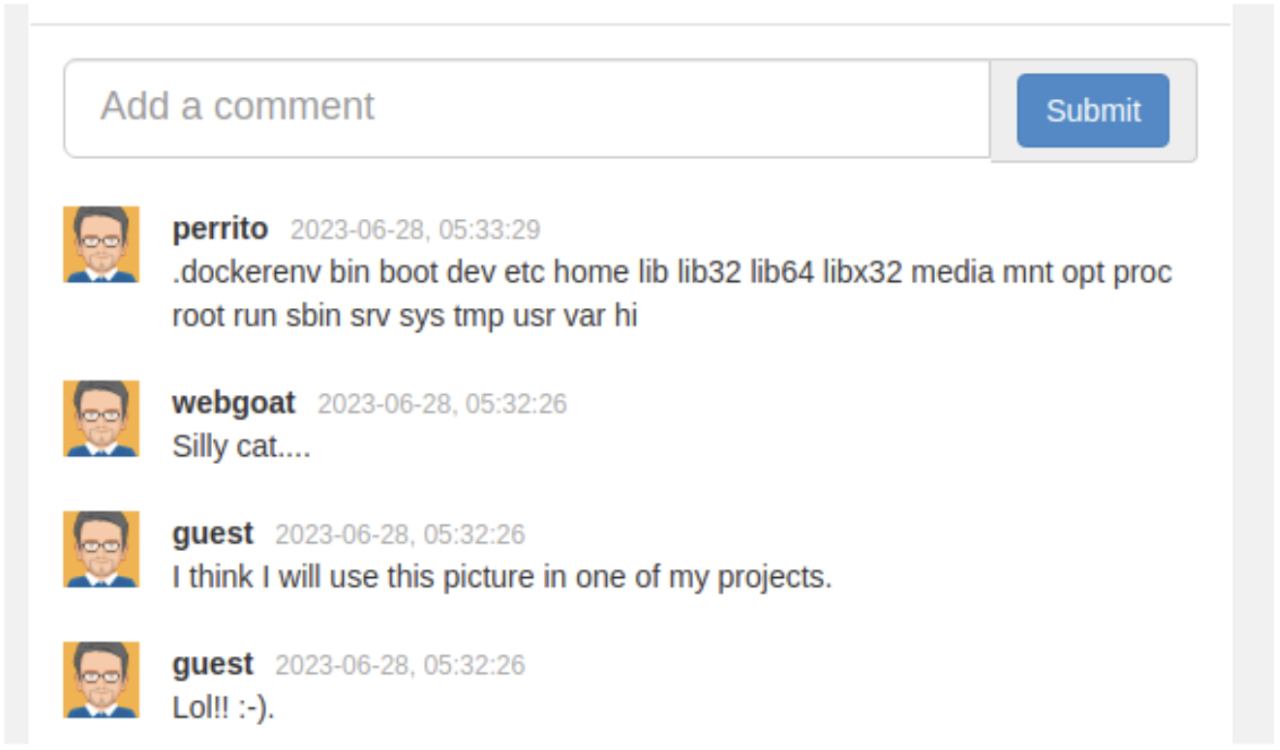
\includegraphics[width=12cm]{img/xxe7.png}
            
            \vspace{0.1em}
            
            Fig. 44: Visualización de directorios de ubicación raíz por pantalla comentarios
        \end{center}
        
        \vspace{2em}





        %%%%%%%%%%%%%%%%%%%%%%%%%%%%%
        %%%% OUTDATED COMPONENTS %%%%
        %%%%%%%%%%%%%%%%%%%%%%%%%%%%%
        \item{\textbf{A6 Vuln and outdated Components}}

        \vspace{1em}

        %%%%%%%%%%%%%%%%%%
        %%%% Módulo 5 %%%%
        %%%%%%%%%%%%%%%%%%
        \textbf{Módulo 5} 
        
        \vspace{1em}
        
        \hspace{20pt}
        En este módulo se plantea documentar la diferencia que existe entre distintas versiones del componente \textit{jquery-ui}. Se trabaja con las versiones \textit{1.10.4} y \textit{1.12.0}. Al inyectar código en la versión vulnerable, que es la versión mas antigua, se obtiene por pantalla el siguiente mensaje:
        
        \vspace{2em}

        \begin{center}
            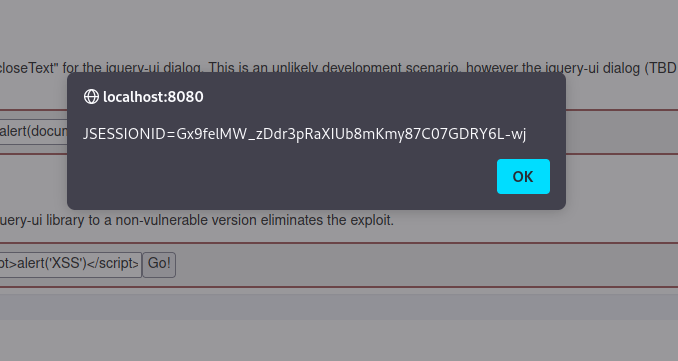
\includegraphics[width=12cm]{img/A6-2.png}
            
            \vspace{0.1em}
            
            Fig. 45: Pop-up message por inyección de script Javascript en versión vulnerable
        \end{center}

        \newpage

        \hspace{20pt}
        Luego, al inyectar código en la versión no vulnerable, que es la versión mas actual, se obtiene por pantalla el siguiente mensaje:
        
        \begin{center}
            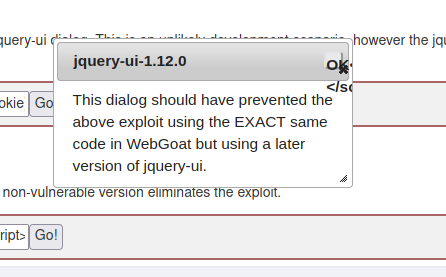
\includegraphics[width=12cm]{img/A6-3.png}
            
            \vspace{0.1em}
            
            Fig. 46: Pop-up message por inyección de script Javascript en versión no vulnerable
        \end{center}

        \vspace{2em}
        




        %%%%%%%%%%%%%%%%%%%%%%%%%%
        %%%% SECURE PASSWORDS %%%%
        %%%%%%%%%%%%%%%%%%%%%%%%%%
        \item{\textbf{A7 Identity and Auth Failure - Secure Passwords}}
        
        \vspace{1em}

        %%%%%%%%%%%%%%%%%%
        %%%% Módulo 4 %%%%
        %%%%%%%%%%%%%%%%%%
        \textbf{Módulo 4} 
        
        \vspace{1em}
        
        ¿Cuánto tiempo podría llevar forzar tu contraseña?
        
        \hspace{20pt}
        En esta tarea, tienes que escribir una contraseña que sea lo suficientemente fuerte (al menos 4/4). Cuando termines, te recomendamos que pruebes algunas de las siguientes contraseñas para ver por qué no son buenas opciones: (password, johnsmith, 2018/10/4, 1992home, abcabc, fffget, poiuz, @dmin).
        
        \vspace{1em}

        \hspace{20pt}
        Utilizando la aplicación web \textit{Diceware Secure Passphare and Password Generator} podemos crear contraseñas criptográficamente fuertes, formadas por frases que contienen una serie de palabras de origen aleatorio.
        
        \newpage
        
        \begin{center}
            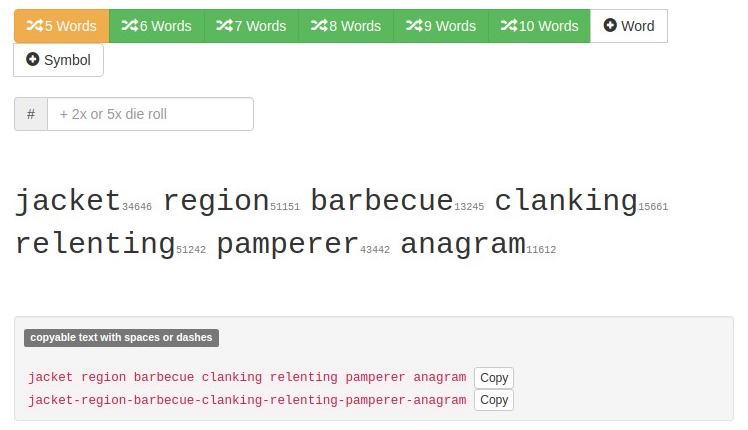
\includegraphics[width=12cm]{img/web-secure-password1.png}
            
            \vspace{0.1em}
            
            Fig. 47: Palabras creadas aleatoriamente formando una frase de seguridad
        \end{center}
        
        \vspace{2em}

        \hspace{20pt}
        Se genera una frase de siete palabras ordenadas aleatoriamente, con dos opciones de separación entre palabra: un espacio o un guión medio. Para realizar la prueba de seguridad en WebGoat se elije la opción con guión medio. Tras ingresar esta opción en la aplicación web, obtenemos el siguiente resultado.
        
        \vspace{2em}
        
        \begin{center}
            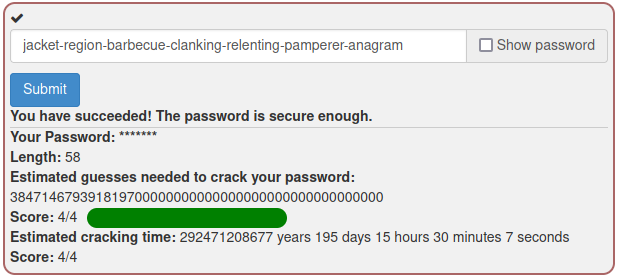
\includegraphics[width=12cm]{img/9.png}
            
            \vspace{0.1em}
            
            Fig. 48: Estadísticas entregadas por WebGoat de la contraseña generada
        \end{center}
        
        \vspace{2em}
        
        \hspace{20pt}
        Por otro lado, se utiliza la aplicación de consola \textit{PWGEN}, la cual permite generar contraseñas aleatorias en base a un bloque de caracteres que ordena de forma aleatoria.

        \newpage
        
        \begin{center}
            \includegraphics[width=12cm]{img/PWGEN.png}
            
            \vspace{0.1em}
            
            Fig. 49: Contraseña generada por PWGEN
        \end{center}
        
        \vspace{2em}
        
        \hspace{20pt}
         El parámetro \textit{-s} genera una contraseña totalmente aleatoria basada en letras y números. \textit{-c} permite que se incluya aleatoriamente al menos una letra en mayúscula. \textit{-B} elimina caracteres ambiguos en la generación. Con \textit{20} se indica una longitud de contraseña de 20 caracteres. Finalmente, con el parámetro \textit{1} se le indica que solo se requiere la generación de una contraseña.
         
        \vspace{1em}
        
        Al ingresar este resultado en WebGoat se obtiene el siguiente resultado:

        \vspace{2em}
        
        \begin{center}
            \includegraphics[width=12cm]{img/8.png}
            
            \vspace{0.1em}
            
            Fig. 50: Estadísticas entregadas por WebGoat de la contraseña generada por PWGEN
        \end{center}
        
        \vspace{2em}

        \hspace{20pt}
        Finalmente, se realizan pruebas con una de las contraseñas indicadas al comienzo del ejercicio con el fin de destacar la diferencia entre una contraseña segura y una que no lo es, ante el descubrimiento de esta por fuerza bruta. Se utiliza la opción \textit{2018/10/4}.

        \newpage
        
        \begin{center}
            \includegraphics[width=12cm]{img/3.png}
            
            \vspace{0.1em}
            
            Fig. 51: Estadísticas entregadas por WebGoat de la contraseña planteada en ejercicio
        \end{center}
        
        \vspace{2em}

        \hspace{20pt}
        Se aprecia la enorme diferencia entre los resultados, en donde se nos indica en el último caso un tiempo estimado de tan solo 48 minutos aproximadamente para obtener la contraseña mediante la aplicación de fuerza bruta.        
    \end{enumerate}
\end{enumerate}

\vspace{2em}





%%%%%%%%%%%%%%%%%%%%%%%%%%%%%
%%%%%3. Post explotación%%%%%
%%%%%%%%%%%%%%%%%%%%%%%%%%%%%
\phantomsection
\newsection{3. Post-explotación}

\vspace{1em}

\hspace{20pt}
Debido a que este informe sólo contempla las temáticas de Recopilación de Información y Explotación, y que la aplicación web, no se realiza el uso de estos o la post explotación del sistema objetivo.

\newpage





%%%%%%%%%%%%%%%%%%%%%%%%%%%%%%%%%%
%%%%%4. Posibles mitigaciones%%%%%
%%%%%%%%%%%%%%%%%%%%%%%%%%%%%%%%%%
\phantomsection
\newsection{4. Posibles mitigaciones}

\vspace{1em}

\hspace{20pt}
En este apartado se entrega información para generar mejoras a nivel de sistema, con la finalidad de mitigar las vulnerabilidades encontradas. Para esto, se toma ayuda de la información expuesta en el sitio web de \textit{OWASP}, con la cual se podrán plantear algún tipo de soluciones para cada una de las vulnerabilidad tratadas.

\vspace{1em}

\begin{enumerate}
    \begin{enumerate}
        %%%%%%%%%%%%%%%%%%%%%%%
        %%%% SQL Injection %%%%
        %%%%%%%%%%%%%%%%%%%%%%%
        \item{\textbf{SQL Injection}}

        \vspace{1em}

        \hspace{20pt}
        Una SQLi se produce cuando los desarrolladores de software crean consultas dinámicas de bases de datos en base a la concatenación de cadenas que incluyen la entrada proporcionada por el usuario. Por lo tanto, evitar una falla por SQLi en primera instancia se gestiona por: 

        \vspace{1em}
        
        \begin{itemize}
            \item Dejar de escribir consultas dinámicas con concatenación de cadenas.
            \item Evitar que la entrada proporcionada por el usuario que contiene SQL malicioso afecte la lógica de la consulta ejecutada.
        \end{itemize}

        Debido a esto es que para prevenir la inyección de código SQL sobre el input de un sitio o página web se requiere mantener los datos separados de los comandos y las consultas que se ejecutan.

        \vspace{1em}

        \hspace{20pt}
        Los ataques por inyecciones SQL son muy comunes, y esto se debe principalmente a dos factores:

        \vspace{1em}
        
        \begin{itemize}
            \item La prevalencia significativa de vulnerabilidades de inyección SQL.
            \item El atractivo del objetivo el acceso a una base de datos suele generar un interes superior, ya que contiene todos los datos sensibles y críticos del sistema).
        \end{itemize}

        \vspace{1em}
        
        \hspace{20pt}
        Dentro de las principales defensas planteadas para evitar SQLi en una web-app se plantean dos tipos de defensas: las primarios y las adicionales.

        \vspace{1em}
        
        \begin{enumerate}
            \begin{enumerate}
                \begin{enumerate}
                    \item{\textbf{Defensas primarias}}

                    \vspace{1em}
                        
                        \begin{itemize}
                            \item Uso de declaraciones preparadas (con consultas parametrizadas).
                            \item Uso de procedimientos almacenados y correctamente construidos.
                            \item Validación de entrada de la lista de permitidos.
                            \item Escapar de todas las entradas proporcionadas por el usuario a nivel de sentencias.
                        \end{itemize}
                        
                    \vspace{1em}

                    \item{\textbf{Defensas adicionales}}

                    \vspace{1em}
                        
                        \begin{itemize}
                            \item Hacer uso del privilegio mínimo al momento del desarrollo de un servicio.
                            \item Realización de la validación de las sentencias de entrada en la lista de permitidos.
                        \end{itemize}
                        
                    \vspace{1em}
                    
                \end{enumerate}
            \end{enumerate}
        \end{enumerate}

        \vspace{1em}

        \hspace{20pt}
        Además, como recomendaciones generales para evitar SQLi en un sitio se tiene:

        \vspace{1em}
        
        \begin{itemize}
            \item La opción preferida es usar una API segura, que evita usar el intérprete por completo, proporciona una interfaz parametrizada o migra a herramientas de mapeo relacional de objetos (ORM).
            \item Utilice una validación de entrada positiva del lado del servidor. Esta no es una defensa completa ya que muchas aplicaciones requieren caracteres especiales, como áreas de texto o API para aplicaciones móviles.
            \item Para cualquier consulta dinámica residual, escape los caracteres especiales usando la sintaxis de escape específica para ese intérprete.
            \item Utilice LIMIT y otros controles de SQL dentro de las consultas para evitar la divulgación masiva de registros en caso de inyección de SQL.   
        \end{itemize}

        \vspace{2em}
        
        %%%%%%%%%%%%%%%%%%%%%%%%%%%%%%
        %%%% Cross Site Scripting %%%%
        %%%%%%%%%%%%%%%%%%%%%%%%%%%%%%
        \item{\textbf{Cross Site Scripting}}

        \vspace{1em}

        \hspace{20pt}
        Una vulnerabilidad Cross-Site Scripting (XSS) es un tipo de inyección, en el que se inyectan scripts maliciosos en sitios web. Los ataques XSS ocurren cuando un atacante usa una aplicación web para enviar código malicioso, generalmente en forma de un script del lado del navegador, a un usuario final diferente. Las fallas que permiten que estos ataques tengan éxito están bastante extendidas y ocurren en cualquier lugar donde una aplicación web use la entrada de un usuario dentro de la salida que genera sin validarla o codificarla.

        \newpage

        \hspace{20pt}
        La prevención de XSS requiere la separación de los datos que no son de confianza del contenido activo del navegador. Esto se puede lograr mediante:

        \vspace{1em}

        \begin{itemize}
            \item El uso de marcos que escapan automáticamente de XSS por diseño, como el último Ruby on Rails, React JS.
            \item Escapar los datos de solicitud HTTP que no son de confianza según el contexto en la salida HTML (cuerpo, atributo, JavaScript, CSS o URL) resolverá las vulnerabilidades de XSS reflejadas y almacenadas.
            \item La aplicación de codificación es sensible al contexto tras modificar el documento del navegador en el lado del cliente. Cuando esto no se puede evitar, se pueden aplicar técnicas de escape sensibles al contexto similares a las API del navegador.
            \item Habilitar una política de seguridad de contenido (CSP) como un control de mitigación de defensa en profundidad contra XSS. Es efectivo si no existen otras vulnerabilidades que permitirían colocar código malicioso a través de archivos locales incluidos (por ejemplo, sobrescrituras de recorrido de ruta o bibliotecas vulnerables de redes de entrega de contenido permitidas).
        \end{itemize}

        \vspace{2em}

        %%%%%%%%%%%%%
        %%%% XXE %%%%
        %%%%%%%%%%%%%
        \item{\textbf{Security Misconfiguration}}

        \vspace{1em}

        \hspace{20pt}
        La vulnerabilidad de Error de Configuración de Seguridad se refiere a una incorrecta configuración de los controles de seguridad en un sistema o aplicación. Esto puede permitir que un atacante acceda a información sensible o realice acciones no autorizadas en el sistema desde la aplicación. Estos errores pueden incluir permisos de archivo y directorio incorrectos, configuraciones de cortafuegos deficientes, configuraciones débiles de autenticación o encriptación, entre otros. La explotación de estas vulnerabilidades puede resultar en fugas de datos, compromiso de cuentas de usuario, acceso no autorizado al sistema o manipulación de la aplicación.

        \vspace{1em}

        \hspace{20pt}
        Para prevenir de alguna forma la explotación de esta vulnerabilidad, se deben implementar procesos de instalación seguros de sistemas, ante los cuales podemos ver encontrar algunos de los siguientes puntos:

        \begin{itemize}
            \item Un proceso de endurecimiento repetible hace que sea rápido y fácil implementar otro entorno que esté debidamente bloqueado. Los entornos de desarrollo, control de calidad y producción deben configurarse de manera idéntica, con diferentes credenciales utilizadas en cada entorno. Este proceso debe automatizarse para minimizar el esfuerzo requerido para configurar un nuevo entorno seguro.
            \item Una plataforma mínima sin características, componentes, documentación ni muestras innecesarias. Elimine o no instale características y marcos no utilizados.
            \item Una tarea para revisar y actualizar las configuraciones correspondientes a todas las notas de seguridad, actualizaciones y parches como parte del proceso de administración de parches, por ejemplo mediante tareas cron programadas con anterioridad.
            \item Una arquitectura de aplicaciones segmentada proporciona una separación eficaz y segura entre componentes o inquilinos, con segmentación, o grupos de seguridad 
            \item Envío de directivas de seguridad a los clientes como encabezados de seguridad.
            \item Un proceso automatizado para verificar la eficacia de las configuraciones y ajustes de todos los entornos.
        \end{itemize}

        \vspace{2em}

        %%%%%%%%%%%%%%%%%%%%%%%%%%%%%%%%%%%%%%%%%%%%
        %%%% Vulnerable and Outdated Components %%%%
        %%%%%%%%%%%%%%%%%%%%%%%%%%%%%%%%%%%%%%%%%%%%
        \item{\textbf{Vulnerable and Outdated Components}}

        \vspace{1em}

        \hspace{20pt}
        La vulnerabilidad de Componentes Vulnerables y Obsoletos hace referencia al uso de versiones desactualizadas o con fallos de componentes de software de u servicio o aplicación. Detro de estos componentes se incluyen bibliotecas, frameworks o plugins. Si estos componentes no se actualizan a sus últimas versiones, pueden contener vulnerabilidades conocidas que los atacantes aprovechan para comprometer la seguridad del sistema. Es importante mantener actualizados los componentes utilizados en las aplicaciones, ya que estas incluyen generalmente correcciones de seguridad para prevenir la explotación de vulnerabilidades conocidas presentes en estas. De lo contrario, los componentes obsoletos pueden ser un punto débil en la seguridad de la aplicación.

        \vspace{1em}

        \hspace{20pt}
        Para prevenir de alguna forma la explotación de esta vulnerabilidad, se plantean algunos puntos recomendables a continuación:

        \vspace{1em}

        \begin{itemize}
            \item Elimine las dependencias no utilizadas, las funciones, los componentes, los archivos y la documentación innecesarias a nivel de sistema.
            \item Haga un inventario continuo de las versiones de los componentes del lado del cliente y del lado del servidor que permite su aplicación (por ejemplo, frameworks ó bibliotecas) y sus dependencias utilizando herramientas como versiones, OWASP Dependency Check, retire.js, etc.
            \item Monitorear continuamente fuentes como Common Vulnerability and Exposures (CVE) y National Vulnerability Database (NVD) para vulnerabilidades en los componentes. Utilice herramientas de análisis de composición de software para automatizar este proceso y mantener actualizadas estas listas. proceso.
            \item Solo obtenga componentes y software de fuentes oficiales a través de enlaces seguros. Prefiera los paquetes firmados para reducir la posibilidad de incluir un componente malicioso modificado.
            \item Supervise las bibliotecas y los componentes que no reciben mantenimiento continuamente o que no crean parches de seguridad para versiones anteriores. Si no es posible aplicar parches, considere implementar un parche virtual para monitorear, detectar o proteger el sistema contra el problema descubierto.
        \end{itemize}

        \vspace{2em}

        %%%%%%%%%%%%%%%%%%%%%%%%%%%%%%%%%%%%%%%%%%%%%%%%%%%%
        %%%% Identification and Authentication Failures %%%%
        %%%%%%%%%%%%%%%%%%%%%%%%%%%%%%%%%%%%%%%%%%%%%%%%%%%%
        \item{\textbf{Vulnerable and Outdated Components}}

        \vspace{1em}

        \hspace{20pt}
        La vulnerabilidad Fallas de identificación y autenticación se refiere a debilidades en los mecanismos de identificación y autenticación de un sistema o aplicación. Este tipo de fallas pueden permitir que los atacantes evadan los controles de acceso y puedan ingresar de manera no autorizada a cuentas o funcionalidades protegidas. Esto puede incluir contraseñas débiles, procesos de autenticación inseguros, falta de verificación de credenciales o gestión inadecuada de sesiones. Las fallas en la identificación y autenticación pueden resultar en violaciones de la privacidad, usurpación de identidad, acceso no autorizado a información sensible o manipulación de datos. Es crucial implementar prácticas de identificación y autenticación seguras para mitigar estas vulnerabilidades.

        \vspace{1em}

        \hspace{20pt}
        Para prevenir de alguna forma la explotación de esta vulnerabilidad, se plantean algunos puntos recomendables a continuación:

        \vspace{1em}

        \begin{itemize}
            \item Siempre que sea posible, implemente la autenticación multifactor para evitar el relleno automatizado de credenciales, la fuerza bruta y los ataques de reutilización de credenciales robadas.
            \item No envíe ni implemente solicitudes con ninguna credencial predeterminada, especialmente para los usuarios administradores.
            \item Implemente comprobaciones de contraseñas débiles, como probar contraseñas nuevas o modificadas en la lista de las 10000 peores contraseñas.
            \item Alineé las políticas de longitud, complejidad y rotación de contraseñas con las pautas del Instituto Nacional de Estándares y Tecnología (NIST) 800-63b en la sección 5.1.1 para secretos memorizados u otras políticas de contraseñas modernas basadas en evidencia.
            \item Asegúrese de que las rutas de registro, recuperación de credenciales y API estén protegidas contra los ataques de enumeración de cuentas mediante el uso de los mismos mensajes para todos los resultados.
            \item Limite o retrase cada vez más los intentos de inicio de sesión fallidos, pero tenga cuidado de no crear un escenario de denegación de servicio hacia el servidor. Registre todos los errores que se produzcan y alerte a los administradores cuando se detecten ataques de Credential Stuffing, fuerza bruta u otros.
            \item Utilice un administrador de sesión incorporado, seguro y del lado del servidor que genera una nueva ID de sesión aleatoria con alta entropía después de iniciar sesión. El identificador de sesión no debe estar en la URL, almacenarse de forma segura e invalidarse después de los tiempos de espera de cierre de sesión, inactividad y absoluto, con el fin de no generar lecturas por pantalla de los cookies de sesión.
        \end{itemize}

    \end{enumerate}
\end{enumerate}

\newpage





%%%%%%%%%%%%%%%%%%%%%%%%%%%%%%%%%%%%%%%%%%%%%%%%%%%%%%%
%%%%%5. Herramientas utilizadas durante el proceso%%%%%
%%%%%%%%%%%%%%%%%%%%%%%%%%%%%%%%%%%%%%%%%%%%%%%%%%%%%%%
\phantomsection
\newsection{5. Herramientas utilizadas}

\vspace{1em}

\hspace{20pt}
Para el desarrollo de la presente auditoría se utilizaron una serie de herramientas, con el fin de gestionar de mejor forma la información obtenida durante el procedimiento y poder depurar esta de una mejor manera. A continuación se presenta una breve descripción de cada una de ellas, y una referencia al lugar de la auditoría en donde fueron  utilizadas.

\vspace{1em}

\begin{enumerate}
    \begin{enumerate}
        
        %%%%%%%%%%%%%%%%%%
        %%%% nslookup %%%%
        %%%%%%%%%%%%%%%%%%
        \item{\textbf{NSLOOKUP}}

        \vspace{1em}

        \hspace{20pt}
        \textit{NSLOOKUP} es una herramienta de línea de comandos, utilizada tanto en sistemas UNIX como en sistemas Windows, cuya función principal es encontrar la dirección IP de un equipo en concreto, y gracias a esto entregarnos información del DNS de este objetivo. Obtiene directamente la información solicitada sobre el servicio mediante la caché del DNS de este servidor. 

        \vspace{1em}

        \hspace{20pt}
        Como usuarios disponemos de dos modos para utilizar esta herramienta: un modo \textit{no interactivo}, centrado en inspeccionar las entradas de la memoria caché del DNS objetivo almacenadas en el DNS local (modo recomendado para peticiones o solicitudes sencillas, en la que se busca una única entrada para un dominio específico dentro del DNS local). En caso de realizar solicitudes mas complejas haciendo referencia a otro servidor DNS que no sea el local, será necesario utilizar el modo \textit{interactivo}, el cual permite interactuar mediante una interfaz de comandos propia de nslookup por separado de la shell nativa en que se ejecuta el programa.

        \vspace{1em}

        \hspace{20pt}
        Para obtener mas información sobre esta herramienta, como el detalle de los argumentos y flags que se pueden utilizar para realizar las peticiones, se pueden acceder al manual del programa en sistemas Unix, mediante el comando \textit{man nslookup}, o desde la ruta \textit{/usr/share/man}.

        \vspace{1em}

        \hspace{20pt}
        En este informe se utiliza para obtener mas información del DNS del sistema objetivo. Dado que el entorno a vulnerar es precisamente un entorno local, la información obtenida corresponde a la de nuestro propio sistema.
        
        \vspace{2em}

        %%%%%%%%%%%%%%%%%%%%
        %%%% Wappalyzer %%%%
        %%%%%%%%%%%%%%%%%%%%
        \item{\textbf{Wappalyzer}}

        \vspace{1em}

        \hspace{20pt}
        \textit{Wappalyzer} es una herramienta de análisis de tecnologías web, utilizada para identificar las técnicas dispuestas en el desarrollo de un sitio o página web. Proporciona información detallada sobre el software y los servicios utilizados, incluyendo el sistema de gestión de contenido (CMS), el framework web, el servidor web, el lenguaje de programación, las bibliotecas JavaScript, entre otros.
        
        \vspace{1em}
        
        \hspace{20pt}
        Wappalyzer funciona mediante la detección de huellas digitales y patrones específicos en el código fuente, las solicitudes HTTP y otros elementos de un sitio web. Esta información es útil para desarrolladores, investigadores y profesionales de seguridad que desean obtener una comprensión más profunda de las tecnologías implementadas en un sitio o página web.

        \vspace{1em}

        \hspace{20pt}
        En este informe es utilizada para obtener información detallada sobre las tecnologías presentes en el servicio WebGoat.

        \vspace{2em}

        %%%%%%%%%%%%%%
        %%%% NMAP %%%%
        %%%%%%%%%%%%%%
        \item{\textbf{NMAP}}

        \vspace{1em}

        \hspace{20pt}
        \textit{Nmap} o \textit{Network Mapper} es una poderosa herramienta de exploración y descubrimiento de redes utilizada en sistemas Windows, pero por sobre todo en Linux. Su función principal es escanear y mapear redes, identificando hosts activos, puertos abiertos, servicios en ejecución, información de versiones, entre otras.
        
        \vspace{1em}

        \hspace{20pt}
        Nmap utiliza técnicas de escaneo avanzadas como los escaneos de puertos TCP ó UDP, versiones de servicios, sistemas operativos y detección de firewalls. Estas capacidades permiten a un profesional de ciberseguridad obtener una visión completa de la red objetivo y los sistemas que se están evaluando.

        \vspace{1em}

        \hspace{20pt}
        Esta herramienta es utilizada para diversos propósitos, como auditorías de seguridad, evaluaciones de vulnerabilidades, descubrimiento de hosts en una red específica, administración de redes y detección / solución de problemas. Ayuda a identificar puertos abiertos que podrían ser explotados por un atacantes, descubrir servicios y versiones desactualizadas que representan riesgos de seguridad para un sistema en particular, y proporcionar información valiosa para asegurar y mejorar la infraestructura de una red.

        \vspace{1em}

        \hspace{20pt}
        Nmap es ejecutada desde línea de comandos y ofrece una amplia gama de opciones y funcionalidades configurables. Puede realizar escaneos rápidos y básicos para obtener una visión general rápida de la red, o realizar escaneos exhaustivos y detallados de esta, para obtener información más precisa y completa.
        
        \vspace{1em}

        \hspace{20pt}
        Para obtener mas información sobre esta herramienta, se pueden acceder al manual del programa en sistemas Unix, mediante el comando \textit{man nmap}.

        \vspace{1em}

        \hspace{20pt}
        En este informe nmap es utilizado para obtener información sobre los servicios que corren en el sistema objetivo y sus respectivas versiones, los puertos que se encuentran abiertos y el sistema operativo bajo el que se ejecuta WebGoat.

        \vspace{2em}

        %%%%%%%%%%%%%%%%%%%
        %%%% BURPSUITE %%%%
        %%%%%%%%%%%%%%%%%%%
        \item{\textbf{BURPSUITE}}

        \vspace{1em}

        \hspace{20pt}
        \textit{Burp Suite} es una herramienta  de seguridad de aplicaciones web utilizada principalmente en sistemas Linux. Es reconocida en la industria de la seguridad por su alta y completa funcionalidad, y su amplio conjunto de características internas que presenta. Burp Suite se utiliza para evaluar la seguridad de aplicaciones web al identificar y explotar vulnerabilidades potenciales que estas presentan.

        \vspace{1em}

        \hspace{20pt}
        Una de las funcionalidades principales que BurpSuite ofrece es el interceptador de proxy, el cual nos permite interceptar y modificar el tráfico entre el cliente y el servidor web. Esto facilita la identificación de vulnerabilidades como inyecciones SQL, cross-site scripting (XSS), falsificación de solicitudes entre sitios (CSRF), XML external entity (XXE) y más. Además, proporciona una extensa biblioteca de herramientas de escaneo, como el escáner de vulnerabilidades, que ayuda a identificar de manera automatizada posibles problemas de seguridad de una aplicación web.

        \vspace{1em}

        \hspace{20pt}
        Por otro lado, incluye características avanzadas para realizar pruebas de autenticación, manipulación de cookies, generación de pruebas de estrés y secuenciación de ataques. Esto genera la posibilidad de que los profesionales de seguridad puedan simular y evaluar diversos escenarios de ataque en entornos controlados.

        \vspace{1em}

        \hspace{20pt}
        En este informe Burpsuite es utilizado para realizar el secuestro de solicitudes entre la comunicación del cliente y el servidor, con el fin de realizar modificaciones sobre estas y descubirir posibles vulnerabilidades en el sistema objetivo.

        \newpage

        %%%%%%%%%%%%%%%%%%%%%%%%%%%
        %%%% DEVELOPMENT TOOLS %%%%
        %%%%%%%%%%%%%%%%%%%%%%%%%%%
        \item{\textbf{Development Tools}}

        \vspace{1em}

        \hspace{20pt}
        Las herramientas de desarrollo de un navegador son conjuntos de utilidades y funciones integradas en los navegadores web modernos que permiten analizar, depurar y optimizar aplicaciones y sitios web.

        \vspace{1em}

        \hspace{20pt}
        Estas herramientas proporcionan una interfaz de usuario que permite inspeccionar y manipular el código HTML, CSS y JavaScript en tiempo real, lo cual da la posibilidad de comprender la estructura de la página, realizar cambios en el diseño y comportamiento, y depurar posibles errores.

        \vspace{1em}

        \hspace{20pt}
        Además de la inspección de código, las herramientas de desarrollo también ofrecen funciones de seguimiento y visualización de redes, con las cuales se puede monitorear las solicitudes y respuestas del servidor, analizar los tiempos de carga de los recursos y detectar posibles problemas de rendimiento.

        \vspace{1em}

        \hspace{20pt}
        En este informe, las herramientas de desarrollador utilizadas son \textit{NETWORK}, con el fin de captar la presencia de solicitudes entre cliente y servidor y obtener información como las cookies de sesión, y \textit{CONSOLE}, la cual permite realizar inyección de comandos Javascript para obtener cierto tipo de respuesta por el output de esta.
        
        \vspace{2em}

    \end{enumerate}
\end{enumerate}
        

\vspace{2em}

\end{document}

%%%%%%%%%%%%%%%%%%%%%%%%%%%%%%%%%%%%%%%%%
%%%%%          END CONTENTS         %%%%%
%%%%%%%%%%%%%%%%%%%%%%%%%%%%%%%%%%%%%%%%%